\documentclass{sigmod08}
\usepackage{graphicx}
\usepackage{times}
\usepackage{color}
\usepackage{graphicx}
\usepackage{latexsym}
\usepackage{url}
\usepackage{xspace}
\usepackage{boxedminipage}
\usepackage{subfigure}
\usepackage{floatflt}
\usepackage{cite}
\newtheorem{theorem}{Theorem}[section]
\newtheorem{lemma}[theorem]{Lemma}
\newtheorem{proposition}[theorem]{Proposition}
\newtheorem{corollary}[theorem]{Corollary}
\newtheorem{hypothesis}{Hypothesis}
\newtheorem{definition}{Definition}

%% BOON STUFF
\renewcommand{\ttdefault}{cmtt}
\newcommand{\dataloglabel}[1]{\mbox{\bf #1:}\hfil}
\newenvironment{datalog}
  {\begin{list}{}%
      {\it \small \renewcommand{\makelabel}{\dataloglabel}%
    \setlength{\parsep}{-2pt}%
    }%
  }%
{\end{list}}
\newcommand{\datalogspace}{\textcolor[gray]{1}{.}\hspace{0.5in}}
\def\link{\texttt{\#link}\xspace}
\newcommand{\term}[1]{\textbf{#1}}

\newcommand{\ol}[1]{\texttt{\small #1}\xspace}

% Compact itemize and enumerate. Note that they use the same counters and
% symbols as the usual itemize and enumerate environments.
\def\compactify{\itemsep=0pt \topsep=0pt \partopsep=0pt \parsep=0pt}
 \let\latexusecounter=\usecounter
 \newenvironment{CompactItemize}
   {\def\usecounter{\compactify\latexusecounter}
    \begin{itemize}}
   {\end{itemize}\let\usecounter=\latexusecounter}
 \newenvironment{CompactEnumerate}
   {\def\usecounter{\compactify\latexusecounter}
    \begin{enumerate}}
   {\end{enumerate}\let\usecounter=\latexusecounter}
   
   %\newcommand{\jmh}[1]{{\textcolor{red}{#1 -- JMH}}}
   %\newcommand{\jmh}[1]{{}}
   %\newcommand{\petros}[1]{{[\textcolor{green}{#1 -- PM}]}}
   %\newcommand{\petros}[1]{{}}
   \newcommand{\eat}[1]{}

\newcommand{\stitle}[1]{\textbf{#1}---}

\begin{document}
%
% --- Author Metadata here ---
%\conferenceinfo{Under Submission}{}
\toappear{Under Submission}
%\setpagenumber{50}
%\CopyrightYear{2002} % Allows default copyright year (2002) to be over-ridden - IF NEED BE.
%\crdata{0-12345-67-8/90/01}  % Allows default copyright data (X-XXXXX-XX-X/XX/XX) to be over-ridden.
% --- End of Author Metadata ---

% ****************** TITLE ****************************************

\title{Evita Raced: Metacompilation for Declarative Networks\\
{\large Under Submission. Please do not redistribute}}

% ****************** AUTHORS **************************************

\numberofauthors{3}
\author{
\alignauthor Tyson Condie\\
\affaddr UC Berkeley
\alignauthor Joseph M. Hellerstein\\
\affaddr UC Berkeley
\alignauthor Petros Maniatis\\
\affaddr Intel Research Berkeley
% You can go ahead and credit any number of authors here,
% e.g. one 'row of three' or two rows (consisting of one row of three
% and a second row of one, two or three).
%
% The command \alignauthor (no curly braces needed) should
% precede each author name, affiliation/snail-mail address and
% e-mail address. Additionally, tag each line of
% affiliation/address with \affaddr, and tag the
% e-mail address with \email.
%
% 1st. author
}

\maketitle

\begin{abstract}
There has been renewed interest in recent years in applying declarative languages to new application domains outside of traditional data management.  Since these are relatively early research efforts, it is important that the architectures of these new declarative systems be extensible, in order to accommodate unforeseen needs in these new domains.  In this paper, we apply the lessons of declarative systems to the {\em internals} of a declarative networking engine.  Specifically, we describe our design and implementation of {\em Evita Raced}, an extensible query optimizer for the Overlog language used by the P2 declarative networking system.  Evita Raced is a {\em metacompiler}: an Overlog compiler written in Overlog.  We describe the architecture of Evita Raced, including its extensibility interfaces and its dataflow-based runtime structure.  We demonstrate that a declarative language like Overlog is well-suited to expressing traditional and novel query optimizations, in a compact and natural fashion.  Finally, we present initial results of Evita Raced extended with various optimization programs, running on both Internet overlay networks and wireless sensor networks.

% Distributed query processing is a primary bottleneck in many applications that interpret data distributed over a large set of machines.  The distributed query engine component is often part of the application code base,  and finely tuned to handle a very specific workload and network topology. Performance suffers when assumptions about the data or system state deviate from the norm. Moreover, the distributed query engine logic complicates the application design by incorporating code that queries massive amounts of data spread across a large number of machines.  
% 
% In this paper, we describe the P2 declarative query optimizer meta-compilation framework. The optimization framework is contained within the P2 query processing engine, and it exports an interface for submitting rewrite rules over the logical query plan. A rewrite rule takes the form of a query written in the same declarative language (Overlog) used to submit client queries. The logical query plan of a query is represented by a set of relations, over which the rewrite rules query and update.  In this paper, we show that many traditional database optimizations, like the System R optimization algorithm and the Magic-Set rewrite, can be easily expressed as Overlog queries.  We believe that statistics gathering, for cost based optimization rules, can also be written as Overlog queries over the data and system state, leading to a more adaptive query plan generator. Expressing the optimization algorithms as Overlog queries leads to a more concise representation of the algorithm and a dramatic reduction in the overall coding effort.
 
\end{abstract}

\section{Introduction}
There has been renewed interest in recent years in applying declarative
languages to a variety of applications outside the traditional
boundaries of data management.  Examples include work on
compilers~\cite{lam05context}, computer games~\cite{white-sigmod07}, security
protocols~\cite{li-padl03}, and modular
robotics~\cite{ashley-iros07}. Among the most active of these new areas
is the work on {\em Declarative Networking} initiated by the P2
project~\cite{loo-sigmod06,singh-eurosys06}, and followed on by variety
of recent related
efforts~\cite{chu-sensys07,abadi-netdb07,belaramani-sosp07,soule-sosp07}.
The initial motivation for Declarative Networking came from the
recursive graph-traversals in various network routing protocols, which
are natural to express in recursive query languages like
Datalog~\cite{loo-sigcomm05}.  Subsequently, the argument for the
fitness of declarative languages to networking was expanded to include
the asynchronous message-handling inherent in network protocols: the
case was made that message-handling is compactly expressed as joins of
data streams of messages with persistent though transient ``rendezvous''
or ``session'' state~\cite{loo-sosp05,loo-sigmod06}.  These intuitions
were made concrete via working implementations of complex network
protocols at various levels of the protocol stack, often with
drastically reduced code sizes that were expressed in an intuitive
manner quite similar to protocol inventors'
pseudocode~\cite{loo-sosp05,chu-sensys07}.  


Declarative Networking and related topics have the potential to expand the lessons and impact of database technologies into new domains, while reviving interest in classical database topics like recursive query processing that had received minimal attention in recent years.  Yet surprisingly, the proponents of Declarative Networking have not to date applied their ideas to the design of their own systems: the P2 declarative overlay system is implemented in C++~\cite{loo-sosp05}, and the DSN declarative sensor network system is implemented in an embedded dialect of C~\cite{chu-sensys07}.  This is particularly disappointing given the still-emerging use cases for these systems, which are likely to require the systems to be adjusted to unforeseen requirements.

In this paper, we put declarative systems ``in the mirror,''
investigating a declarative implementation of a key aspect of a
declarative system.  Specifically, we have reimplemented the query
optimizer of P2 as a {\em metacompiler}: a compiler (optimizer) for the
P2 language, Overlog, that is itself written in Overlog.  We call the
resulting implementation ``Evita Raced.''\footnote{``Evita Raced'' is
almost ``Declarative'' in the mirror, but as with the Overlog language
itself, it makes some compromises on complete declarativity.}  Using
Evita Raced, we extended P2 with a number of important query
optimization techniques it formerly lacked, and found that our
declarative infrastructure made this quite elegant and compact. For
example, our implementation of the traditional System R dynamic
programming algorithm comprises only 38 Overlog rules (225 lines of
code); our implementation of the Magic Sets Rewriting optimization for
recursive queries is not only compact (68 rules, 264 lines), but also
nearly a direct translation of the description from Ullman's course
notes on the subject~\cite{ullmanNotes}.   The elegance of our
approach comes in part from the fact that query optimization techniques
-- like many search algorithms -- are at heart recursive algorithms, and
benefit from a declarative approach in much the same way as networking
protocols.  Even non-recursive optimization logic -- such as parts of
Ullman's magic-sets algorithm -- is simple enough to express in a
declarative fashion that abstracts away mechanistic details such as the
scheduling of data-parallel steps (e.g., scanning all rules in a program
in parallel versus sequentially).

Our contributions here are three-fold.  First, we present a declarative
architecture for query optimization that is based on metacompilation,
reusing the query executor in a stylized fashion to serve as the engine beneath the optimization process.  Second, we show that a variety of traditional and novel query optimizations are easy to express in a recursive, declarative language. Finally, we evaluate the simplicity and applicability of our design via a full-fledged implementation of an Overlog query optimizer for the P2 Declarative Networking engine, which also cross-compiles code that runs on the DSN wireless sensor network platform~\cite{chu-sensys07}.  
We also include a discussion of the various compromises that we had to make along the way in the interest of pragmatism.  Despite the various engineering details that arose, we believe that declarative metacompilation is a clean, architecturally parsimonious way to build the next generation of extensible query optimizers, particularly as declarative languages get applied in new domains where the relevant optimizations remain unknown.

\section{P2: Language and Architecture}
\label{sec:arch}
% \jmh{This section's text makes too few assumptions about the audience.  SIGMOD reviewers should be expected to have a good familiarity with a traditional DBMS optimizer and executor, and at least passing familiarity with Datalog.  The terminology here needs to match their expectations, and the section can be made much shorter as well.  Basically focus on the main distinctions between P2 and, say, Oracle or Postgres.  Probably also makes sense to put the language tutorial ahead of the architectural discussion, to motivate things like localization.}
% \jmh{Here's how I envision this section being structured:}
% \begin{itemize}
%     \item Overall Architecture: Locally, a Parser, Optimizer, and Continuous Dataflow Executor with mix of relational and network elements.  Globally, SPMD, and talk about query dissemination/installation.  Big change in this paper: the Optimizer is going to use the Executor as its runtime.
%     \item Overlog introduction. Data model: relations, materialized (soft-state) and streaming. To the extent that it's reasonable, cast Overlog as a Datalog variant.  Present local fixpoint as a ``true'' Datalog kernel, defined on a traditional EDB where there's really no distinction between events, soft-state, or what have you.  All updates and remote IDB deductions are extra-fixpoint activity that set up that EDB.  Any requirements for ECA-like syntax should be cast as internal representations, not a Overlog syntax requirements (this may expand the set of rewrites required.)  Comment on monotonic programs being equivalent to Boon's Network Datalog.  Put example in this subsection.
%     \item Internal representation: ECA rules and their mapping to dataflow strands.  
%     \item The dataflow event loop: specifically how updates/messages are dequeued before/after the atomic fixpoint computation, how the dequeued event drives the strands, and how local loops in the dataflow are handled.
% \end{itemize}
% \jmh{End of proposed structure.}
We begin our discussion with an overview of key aspects of the P2 declarative network system.
While ostensibly a network protocol engine, architecturally P2 resembles a fairly traditional shared-nothing parallel query processor, targeted at both stored state and data streams.  P2 supports a recursive query language called Overlog that resembles traditional Datalog with some extensions we discuss below.  Each P2 node runs the same query engine, and, by default, participates equally in every ``query.''   In parallel programming terms, P2 
supports the  Single-Program-Multiple-Data (SPMD) model of parallel computation.

The P2 runtime at each node consists of a compiler---which parses programs,
optimizes them (minimally), and physically plans them---a dataflow executor, and access methods.  The P2 compiler is 
monolithic and implemented in an imperative language (C++). The subject
of this work is the replacement of this monolithic compiler with a
runtime-extensible compiler framework that admits not only imperative
but also declarative optimizers and other compilation stages.  In this section,
we highlight the distinguishing features of the Overlog language, as
well as the P2 dataflow executor and access methods.

\subsection{Overlog, Revisited}
\label{sec:overlog}
The original paper on P2 presented Overlog in an ad-hoc manner as an event-driven language. Since that time, the P2 group has refined the Overlog language and the P2 runtime semantics a fair bit.  However, the only published discussion of the current state of Overlog is in the tutorial document included with the P2 source distribution, which is also quite informal.

In order to build a new optimizer for P2, we had to work with the P2
developer group and the codebase to get familiar with the semantics of
Overlog as it currently stands. In this Section we overview those
semantics, since they form the setting for our work; we did not attempt
to extend or clean up the language and its semantics in this project (see
Section~\ref{sec:gripes} for some unresolved problems we encountered). 

\begin{figure}
\centering
\begin{boxedminipage}{\linewidth}
\scriptsize{\tt
materialize(link,infinity,infinity,keys(1,2)). \\
materialize(path,1,infinity,keys(1,2,3)). \\
materialize(shortestPath,1,infinity,keys(1,2,3)).\\
\\
link(@"localhost:10000", "localhost:10001").\\
link(@"localhost:10001", "localhost:10002").\\
...\\
\\
r1 path(@X,Y,P,C) :- link(@X,Y,C), P := f\_cons(X,Y). \\
\\
r2 path(@X,Y,P,C) :- \\
\datalogspace link(@X,Z,C1), path(@Z,Y,P2,C2), \\
\datalogspace f\_contains(X,P2) == false, \\
\datalogspace P := f\_cons(X,P2), C := C1 + C2. \\
\\
r4 minCostPath(@X,Y,a\_min<C>) :- \\
\datalogspace path(@X,Y,P,C). \\
\\
r5 shortestPath(@X,Y,P,C) :- \\
\datalogspace minCostPath(@X,Y,C), path(@X,Y,P,C).
}
\caption{\label{fig:overlogSP}Shortest path program in Overlog. \ol{a\_}
prefixes introduce aggregate functions and \ol{f\_} prefixes introduce
built-in functions.}
\end{boxedminipage}
\end{figure}

Overlog is based on the traditional recursive query language, Datalog; we assume a passing familiarity with Datalog in our discussion.  As in Datalog, an Overlog {\em program} consists of a set of deduction {\em rules} that define the set of tuples that can be derived from a base set of tuples called {\em facts}. Each rule has a {\em body} on the right of the \texttt{:-} divider, and a {\em head} on the left; the head represents tuples that can be derived from the body.  The body is a comma-separated list of {\em terms}; a term is either a {\em predicate} (i.e., a relation), a {\em condition} (i.e., a relational selection) or an {\em assignment}~\footnote{Overlog's assignments 
are strictly syntactic replacements of variables with expressions; they
are akin to ``\#define'' macros in C++.}.  An example Overlog program that we will use throughout is shown in Figure~\ref{fig:overlogSP}.  Overlog introduces some notable extensions to Datalog:

\stitle{Horizontal partitioning}Overlog's basic data model consists of
relational tables that are partitioned across the nodes in a P2 network.
Each relation in an Overlog rule must have one attribute that is
preceded by an ``@'' sign.  This attribute is called the {\em location
  specifier} of the relation, and must contain values in the network's
underlying address space (e.g., IP addresses for Internet settings,
802.13.4 addresses for sensor networks, hash-identifiers for code
written atop distributed hash tables, etc.)  Location specifiers specify
the horizontal partitioning of the relation: each tuple is stored at the
address found in its location specifier attribute.  At a given node, we
call a tuple a {\em local tuple} if its location specifier is equal to
the local address.  Network communication is implicit in Overlog: tuples
must be stored at the address in their location specifier, and hence the
runtime engine has to send some of its derived tuples across the network
to achieve this physical constraint.  Loo, et al. provide syntactic tests to
ensure that a set of rules can be maintained partitioned in a manner
consistent with its location specifiers and network
topology~\cite{loo-sigmod06}.


\stitle{Soft State and Events}Associated with each Overlog table is a
``soft-state'' lifetime that determines how long (in seconds) a tuple in
that table remains stored before it is automatically deleted.  Lifetimes
can vary from zero to infinity.  Zero-lifetime tables are referred to as
{\em event} tables, and their tuples are called \emph{events}; all other
tables are referred to as {\em materialized} tables.  Overlog contains a
\ol{materialize} declaration that specifies the lifetime of a
materialized table.  At any instant in time, at any given node in the
network, the contents of the local Overlog ``database'' are considered
to be: (a) the local tuples in materialized tables whose lifetime has
not run out, (b) at most one local event fact across {\em all} event
tables, and (c) any derived local tuples that can be deduced from (a)
and (b) via the program rules.  Note that while (b) specifies that only
one event fact is considered to be live at a time per node, (c) could
include {\em derived} local events, which are considered to be live
simultaneously with the event fact.  This three-part definition defines the semantics for a
single P2 node at a snapshot in time.  P2 has no defined semantics
across time and space (in the network); we describe the relevant operational
semantics of the prototype in Section~\ref{sec:eventloop}.
     
\stitle{Deletions and Updates}Overlog, like SQL, supports declarative
expressions that identify tuples to be deleted in a deferred manner
after query execution completes.  To this end, any Overlog rule in a
program can be prefaced by the keyword \ol{delete}.  The program is run to fixpoint, after which the tuples derived in  {\tt
  delete} rules -- as well as other tuples derivable from those -- are removed
from materialized tables before another
fixpoint is executed. It is also possible in Overlog to specify
updates, but the syntax for doing so is different.  Overlog's {\tt
  materialize} statement supports the specification of a primary key for
each relation.  Any derived tuple that matches an existing tuple on the
primary key is intended to {\em replace} that existing tuple, but
the replacement is separated into an insertion and a deletion: the
deduction of the new fact to be inserted is visible within the current
fixpoint, whereas the deletion of the original fact is deferred until
after the fixpoint is computed.

    \subsubsection{A Canonical Example}
        % \jmh{This subsection is incomplete -- it only talks about basic syntax, not about runtime issues.  Even on the syntax front, it doesn't talk about aggregation.  If we want to save it, we should either move it to a subsubsection of 2.1 (and add aggregation), or overview the dataflow execution of shortest paths here.}
        \label{sec:declnet}


        To illustrate the specifics of Overlog, we briefly revisit a shortest
        paths example (Figure~\ref{fig:overlogSP}), similar to that
        of~\cite{loo-sigmod06}, but with fully-realized Overlog syntax that runs
        in P2.  The three \ol{materialize} statements specify that \ol{link},
        \ol{path} and \ol{bestpath} are all tables with infinite lifetime and
        infinite storage space\footnote{The third argument of P2's table
          definition optionally specifies a constraint on the number of tuples
          guaranteed to be allowed in the relation. The P2 runtime replaces
          tuples in ``full'' tables as needed during execution; replaced tuples
          are handled in the same way as tuples displaced due to primary-key overwrite.}.  
        For each table, the positions of the primary key attributes are noted as well.  
        Rule \ol{r1} can be read as saying ``if there is a link tuple of the form \ol{(X,Y,C)} stored at node \ol{X}, then one can derive the existence of a path tuple \ol{(X,Y,P,C)} at node \ol{X}, where \ol{P} is the output of the function \ol{f\_cons(X,Y)} -- the concatenation of \ol{X} and \ol{Y}.''  
Note that rule \ol{r1} has the same location specifiers throughout, and
        involves no communication.  This is not true of the recursive
        rule \ol{r2}, which connects any \ol{link} tuple at a node
        \ol{X} with any path tuple at a neighboring node \ol{Z}, the
        output of which is to be stored back at \ol{X}. As described in
        the earlier work on P2~\cite{loo-sigcomm05,loo-sigmod06} such
        rules can be easily rewritten so that the body predicates all
        have the same location specifier; the only communication then is
        shipping the results of the deduction to the head relation's
        location specifier.  In Section~\ref{sec:localization} we
        briefly describe how we reimplemented this functionality in a
        \emph{localization} compiler stage written in Overlog, within
        Evita Raced.

        % \jmh{This discussion might make more sense if we show the localized version of this program, particularly if we decide to add a discussion of dataflow in here.}


% In this section we describe the Overlog language and the compilation
% of an Overlog program to an execution plan. Our presentation of Overlog
% will be given in the context of its original purpose; defining network protocols.

\subsection{The P2 Runtime Engine}
The P2 runtime is a dataflow engine that was based on ideas from relational databases and network routers; its scheduling and data hand-off closely resemble the Click extensible router~\cite{click-tocs}.  Like Click, the P2 runtime supports dataflow {\em elements} (or ``operators'') of two sorts: pull-based elements akin to database iterators~\cite{graefe-survey}, and push-based elements as well.  As in Click, whenever a pull-based element and a push-based element need to be connected, an explicit ``glue'' element (either a pull-to-push driver, or a queue element) serves to bridge the two.  More details of this dataflow coordination are presented in the original P2 paper~\cite{loo-sosp05}.

\subsubsection{Dataflow Elements}
The set of elements provided in P2 includes a suite of operators familiar from relational query engines: selection, projection, and in-memory indexes.  P2 supports joins of two relations in a manner similar to the symmetric hash join: it takes an arriving tuple from one relation, inserts it into an in-memory table for that relation, and probes for matches in an access method over the other relation (either an index or a scan).  To this suite, we added sorting and merge-joins, which allow us to explore some traditional query optimization opportunities and trade-offs as discussed in Section~\ref{sec:systemr}.

P2 currently has no support for persistent storage, beyond the ability to read input streams from comma-separated-value files.  Its tables are stored in memory-based balanced trees that are instantiated at program startup; additional such trees are constructed by the planner as secondary indexes to support query predicates.

P2 also provides a number of elements used for networking, which handle issues like packet fragmentation and assembly, congestion control, multiplexing and demultiplexing, and so on; these are composable in ways that are of interest to network protocol designers as discussed in~\cite{condie-hotnets05}.  However, the original P2 query optimizer always assembles these network elements in a fixed manner, and we did not choose to change that code in our work here.  The basic pattern is that each P2 node has a single IP port for communication, and the dataflow graph is ``wrapped'' in elements that handle network ingress with translation of packets into tuples, and network egress with translation of tuples into packets.

\subsubsection{The P2 Event Loop}
\label{sec:eventloop}
The control flow in the P2 runtime is driven by a fairly traditional event loop that responds to any network or timer event by invoking an appropriate dataflow segment to handle the event.

The basic control loop in P2 works as follows:
\begin{CompactEnumerate}
    \item An event is taken from the system input queue, corresponding to a single newly-arrived tuple, which is either an {\em insert} tuple (i.e., the result of a normal deduction) or a {\em delete} tuple (the result of a \ol{delete} rule or a primary-key update).  We will refer to this tuple as the {\em current tuple}.
    \item The value of the system clock is noted in a variable we will call the {\em current time}.  This is the time that will be used to determine the liveness of soft-state tuples.  
    %(Note that any event tuples that arrived previously will no longer be live in any event table, which guarantees the single-event semantics described above.)
    \item The current tuple is, logically, appended to its table.
    \item If the current tuple is an insert tuple, the dataflow corresponding to the Overlog program is initiated and run to a local fixpoint following traditional Datalog semantics, with the following exception: during processing, any non-local derived tuples are buffered in a {\em send queue}, as are any derived tuples to be deleted.
    \item If, instead, the current tuple is a delete tuple, the dataflow
    is run to a local fixpoint, but newly-derived local tuples
    (including the current tuple) are copied to a {\em delete queue},
    and newly-derived non-local tuples are marked as delete tuples
    before being placed in the send queue so as to cascade the deletions
    to remote nodes' databases.
    \item All tuples in the delete queue are deleted from their associated tables, and the delete queue is emptied.
    \item The send queue is flushed across the network, with any local updates inserted into the local input queue.
\end{CompactEnumerate}
Some additional operational details we discovered in P2 are discussed
further in Section~\ref{sec:gripes}.

% Unlike Datalog, Overlog must run in the continuous processing context of networking, over streams of tuples representing system events.  This inherently requires more than the single computation of a fixpoint as described in the Datalog literature. P2 has modified its handling of this issue since the initial paper~\cite{loo-sosp05}. P2 nests a fairly traditional declarative Datalog fixpoint execution within an operationally defined local event loop at each node.  An input queue is kept at each P2 node, to hold tuples that correspond to network messages and clock interrupts.  Each tuple in the queue is tagged with the name of a relation in the schema of the Datalog database. The loop begins by noting the local wall-clock time, and deleting from all tables any tuples whose soft-state lifetime has expired; this includes event tuples from the previous iteration of the loop.  At that point, a tuple is dequeued from the input queue and inserted into its associated table.  At that point, the Overlog program is run  to fixpoint atomically, nearly as if it were a traditional single Datalog program.  One exception to traditional Datalog is the handling of derived tuples with remote location specifiers; these are placed directly into network queues for subsequent processing. Another exception involves rules that have {\em actions} in the head -- these actions can be table insertion or deletion; derived tuples in such rules are also enqueued for subsequent processing.  When fixpoint is reached, the queued network messages are sent to their destinations, and the table actions are carried out on the database.  This completes one iteration of the event loop.

%From this perspective, the P2 runtime looks quite a bit like an Event-Condition-Action system with dataflow underneath: events are provided by the clock and network, conditions are checked via the dataflow engine for matches, which are then converted into actions: network messages to be sent, or table updates to be performed.

% \jmh{This is probably too long.  Also, we need to purge text that was recycled from SOSP.  }
% The design of P2 was inspired by prior work in both databases and
% networking. It is based in large part upon a
% side-by-side comparison between the PIER peer-to-peer query
% engine~\cite{pier-cidr05} and the Click router~\cite{click-tocs}. Like
% PIER, P2 can manage structureddata tuples flowing through a broad
% range of query processing elements, which may accumulate significant
% state and perform substantial asynchronous processing.  Like Click, P2
% stresses high-performance transfers of data units, as well as dataflow
% elements with both ``push'' and ``pull'' modalities. 
% 
% At a coarse grain, P2 in its current state consists of (1) an Overlog
% parser, (2) an Planner that translates Overlog to a runtime dataflow
% plan, and (3) a runtime plan executor.  The
% life of a query is simple: the query is parsed into an internal
% representation, the planner constructs a corresponding dataflow graph
% of elements, and the graph is executed by the runtime until it is
% canceled.  We proceed to overview the components bottom-up; more
% details are given in the P2 SOSP paper~\cite{loo-sosp05}.
% 
% Processing in P2 is handled with a dataflow model inspired by Click
% and PIER.  As in Click, nodes in a P2 dataflow
% graph can be chosen from a set of C++ objects called
% \textit{elements}.  In database systems these are often called
% \textit{operators}, since they derive from logical operators in the
% relational algebra.  Elements have some number of input and output
% \emph{ports}.  An arc in the dataflow graph is represented by a
% binding between an output port on one element and an input port on
% another.  Tuples arrive at the element on input ports, and elements
% emit tuples from their output ports. Handoff of a tuple between two elements takes one
% of two forms, \emph{push} or \emph{pull}, determined when the elements
% are configured into a dataflow graph.   
% 
% P2 provides a number of built in dataflow elements that allow it to
% implement networking and query processing logic.  This includes
% elements for the streaming relational query operators found in most
% database systems, e.g., selection, projection, join, and aggregation.
% It also includes networking elements responsible for socket handling,
% packet scheduling, congestion control, reliable transmission, data
% serialization, and dispatch.  P2 has elements to store incoming tuples in tables, 
% iteratively emit tuples in a table matching a filter expression, and {\em listener}
% elements that are notified whenever a tuple is added or deleted from a
% table. Finally, like Click, P2 includes a collection of general-purpose
% ``glue'' elements, such as a queue, a multiplexer, a round-robin
% scheduler, etc.
% 
% Storage in P2 is currently via a main-memory relational Table
% implementation, named using unique IDs that can be shared between
% different queries and/or dataflow elements.  In-memory indices
% (implemented using standard balanced binary trees) can be attached to
% attributes of tables to enable quick equality lookups.  The current
% in-memory implementation serves the system requirements for implementing
% network overlays and streaming query applications, all of which tend
% to expire tuples from memory rather than accumulating them
% indefinitely.  P2's event-driven, run-to-completion model obviates the
% need for locking or transaction support, and relatively simple indices
% suffice to meet performance requirements.  We plan additional
% table implementations that use stable storage for persistent data
% storage; that engineering task is relatively straightforward, but not
% within the scope of this paper.
% 


\section{Declarative Optimization}
\label{sec:declopt}
Evita Raced is a compiler (i.e., query optimizer) for the Overlog
declarative language that supports a runtime-extensible set of program
rewrites and optimizations, which are themselves expressed in Overlog.
This metacompilation approach is achieved by implementing optimization
via dataflow programs  (query plans) running over a set of tables.  Two
main challenges must be addressed to make this work.  First, all
compiler state -- including the internal representation of both
declarative Overlog programs and imperative dataflow programs -- needs
to be captured in a relational representation so that it can be
referenced and manipulated from Overlog.  Second, the (extensible) set
of tasks involved in optimization must itself be coordinated via a
single dataflow program that can be executed by the P2 runtime engine.
In this section we describe the implementation of the Evita Raced
framework, including the schema of the compiler state, the basic
structure of the Evita Raced dataflow graph, and the basic dataflow
fragments needed to bootstrap the optimizer.

% \petros{This paragraph should be an overview of the whole
%   thing. Basically, optimizations and rewrites are themselves P2
%   programs and they can be installed and run while the system itself is
%   already running. What are the challenges? Expressing compilation state
%   like any other regular P2 program's state, and isolating stages,
%   running them in a particular order, etc. Just give a single-paragraph
%   overview. Then there should be a subsection talking about the program
%   representation (what you're talking about in the next two paragraphs
%   and the figtures). }The goal of this work is to be able to express query optimizations and rewrites as Overlog
% programs and have the compiler execute our programs on the input program at 
% specific points in the compilation process. The first challenge that arises is
% how to query and update the internal compiler state (namely the query plan)
% in Overlog. The only state accessible to an Overlog program are the tables defined
% by the system. Therefore, in order to modify compilation state in Overlog, the compiler
% state must be stored in relational format. 

\begin{figure}
\begin{center}
%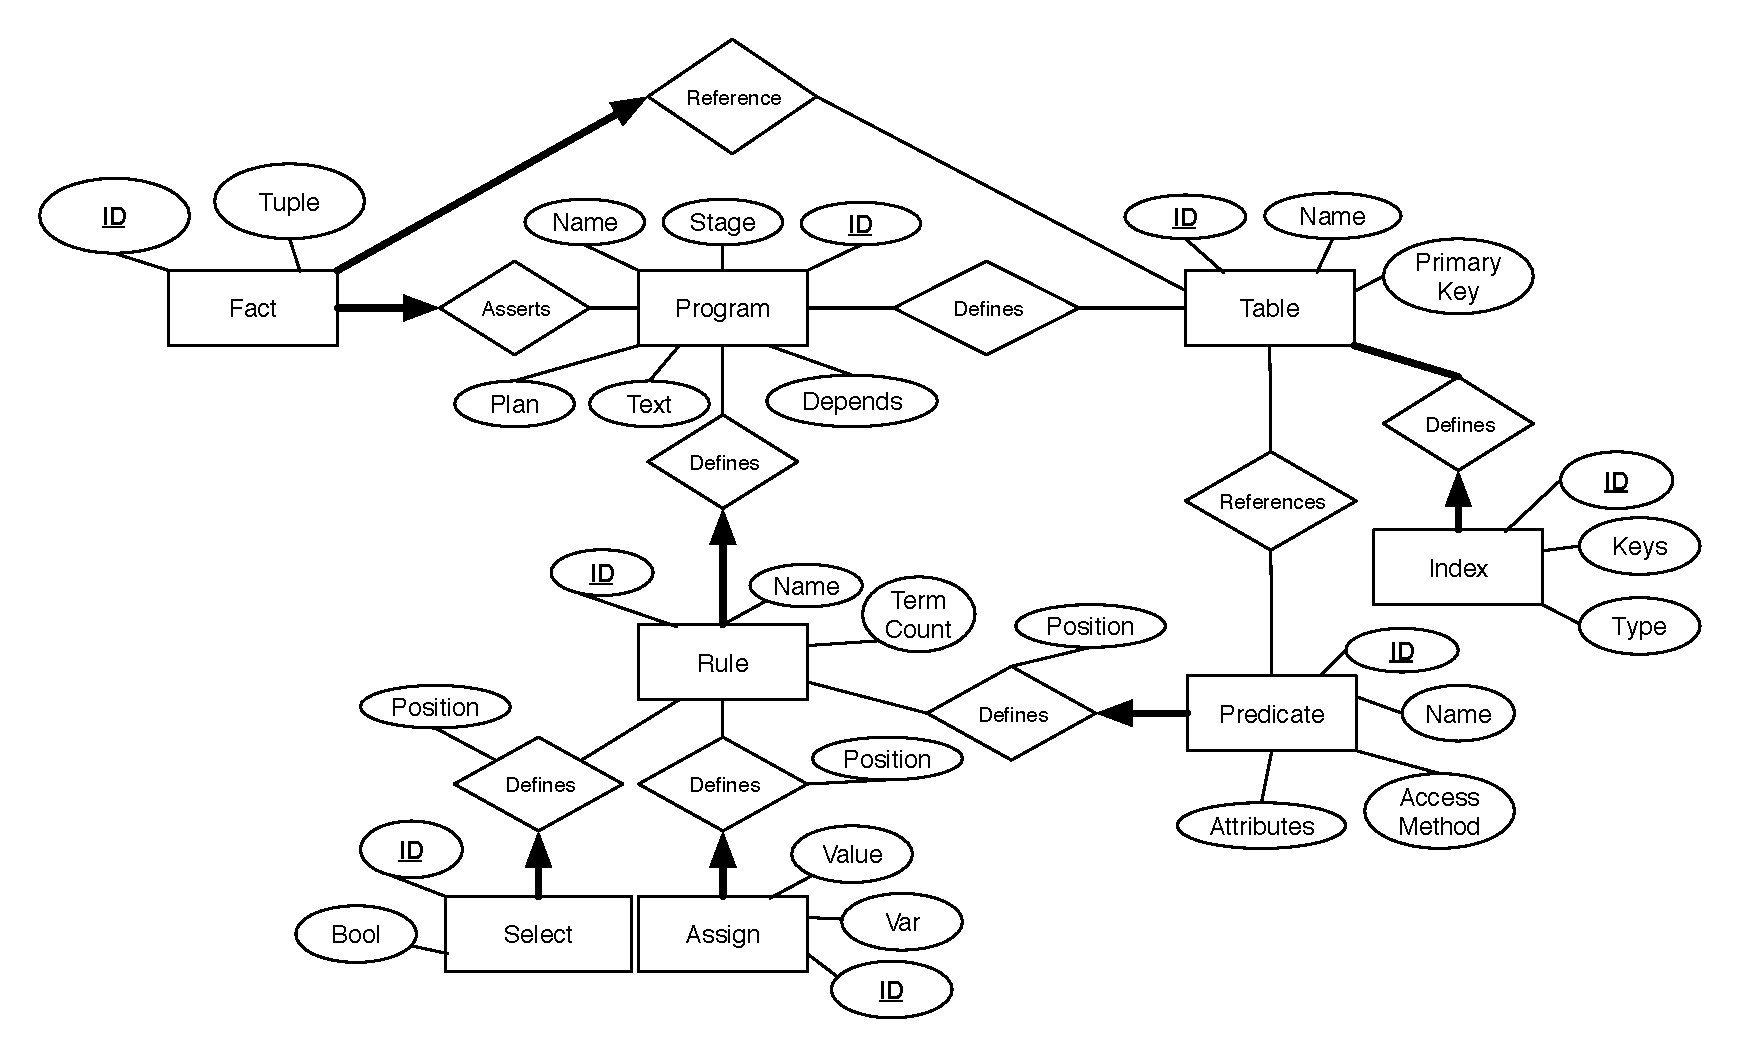
\includegraphics[width=80mm]{p2_er}
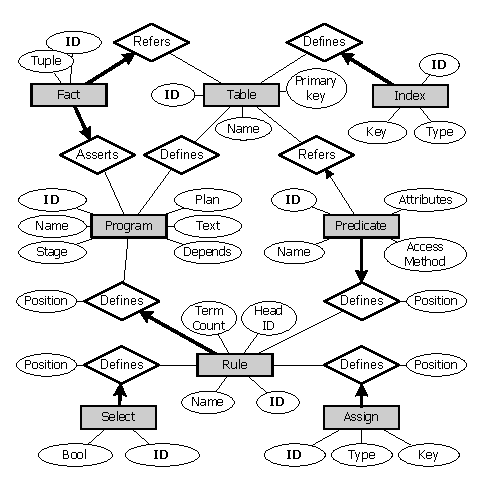
\includegraphics{visio/ERDiagram}
\caption{{ER Diagram of a query plan in P2.}}
\label{fig:p2er}
\end{center}
\end{figure}
\subsection{Table-izing Optimizer State}
A typical query optimizer maintains a number of data structures to describe the contents of a query, and to represent ongoing properties of a query planner including fragments of query plans.  Our first task in designing Evita Raced was to capture this information in a relational schema.

Figure~\ref{fig:p2er} shows an Entity-Relationship diagram we developed that captures the properties of an Overlog program, and its associated P2 dataflow query plans. 
% The entities
% in the diagram represent the components that make up the program and plans, and the
% relationships capture the program structure. 
We derived the constraints in the diagram by reviewing the semantic analysis rules enforced in the original P2 compiler; we discuss a few of them here for illustration.
An Overlog {\em rule} must appear in exactly one {\em program}. 
A {\em select} 
term (e.g., \ol{f\_contains(X,P2) == false} in Figure~\ref{fig:overlogSP}) is a Boolean expression over attributes in the predicates of the rule, and must appear in exactly one {\em rule}.  
% An {\em assign} term (e.g., \ol{C := C1 + C2} in Figure~\ref{fig:overlogSP}) binds variables to expressions that, when evaluated, yield atomic values; each of these must appear in exactly one rule.
The diagram indicates that a {\em predicate} 
must also appear in a unique {\em rule}, and that it may possibly reference a single {\em table}. A predicate
that references a table is called a {\em table predicate} (or a
\emph{materialized predicate}), while one that does not is called an {\em event predicate}. 
An {\em index} is defined over exactly one {\em table}, and a {\em table} defines at least
one index (namely the primary key index, which P2 always
constructs). Some relations may contain a number of {\em facts} at startup, 
each of which must belong to a single program and must reference a single table.

\begin{table}
\centering
\caption{The Metacompiler Catalog: tables defining an Overlog program and dataflow execution plan.}
\label{tbl:tables}
\small{
\begin{tabular}{|l|l|l|} \hline
{\it Name}& {\it Description} & {\it Relevant attributes} \\ \hline\hline
table     & Table definitions & {\bf table\_id}, primary\_key\\ \hline
index     & Index definitions & {\bf index\_id}, {\bf table\_id}, keys, type \\ \hline
fact      & Fact definitions  & {\bf program\_id}, {\bf table\_id}, {\bf id}, tuple\\ \hline
program   & User program      & {\bf program\_id}, name, stage, text,\\
          & description       & depends, plan \\ \hline
rule      & Rules appearing   & {\bf program\_id}, {\bf rule\_id}, name, \\
          & in a program      & term\_count, head\_id \\ \hline
predicate & Predicates appearing & {\bf id}, {\bf rule\_id}, table\_id, name, \\
          & in a rule         & position, access\_method \\ \hline
select    & Selections        & {\bf id}, {\bf rule\_id}, boolean, position \\
          & appearing in a rule &  \\ \hline
assign    & Assignment statements & {\bf id}, {\bf rule\_id}, variable, \\ 
          & appearing in a rule & value, position \\ \hline
\end{tabular}
}
\end{table}

Having (after some design iterations) constructed the ER diagram, converting it to relational format was
straightforward. Table~\ref{tbl:tables} lists the set of relations that capture the entities 
mentioned in the ER diagram; we refer to this as the {\em Metacompiler Catalog}. We modified P2 to create these tables
at system startup, and they are accessible to any optimization programs that get added to the system. The primary key 
columns are bold in  Figure~\ref{fig:p2er} and Table~\ref{tbl:tables}.
% In addition, there are compiler constraints
% that cannot be captured by key constraints alone. For instance, a rule must contain
% exactly one head and one event predicate. Such checks can be performed by integrity 
% constraints written into the compiler logic (possibly as Overlog programs). 

\subsection{Metacompiler Architecture}
\label{sec:metaarch}
Optimization logic expressed in Overlog is declarative, and Evita Raced realizes this logic by converting it to a dataflow program to be executed by the P2 dataflow subsystem.  In this section we describe how Evita Raced represents query optimization programs as dataflow, and also the way it orchestrates multiple different optimization programs through the P2 dataflow framework.

An optimizer built using Evita Raced is composed of an extensible number of {\em stages}, each of which performs some
compilation task on the input program. One way to write an Evita Raced stage is to construct a dataflow program of one or more P2 elements in C++, and compile the result into the P2 binary; this is how we implement certain base stages required for bootstrapping, as described in Section~\ref{sec:bootstrap}.  However, the power of Evita Raced comes from its support for stages written in Overlog, which, in addition to being compactly expressed in a high-level language, can be loaded into a running P2 installation at any time. 
A stage programmer registers a new stage with Evita Raced by inserting a tuple into the {\em program} relation. 
This tuple contains a unique identifier ($program\_id$), a name
($name$),  a list of stage dependencies ($depends$), and the program
text ($text$). Because the \ol{program} relation is used to convey
partial compilation results from stage to stage as well, \ol{program}
tuples also contain attributes for the name of the compiler stage operating 
on the program ($stage$), and the final physical plan ($plan$), though
these attributes are empty when the programmer first creates the tuple. Section~\ref{sec:stageschedule} describes the
$depends$ attribute, and its use in the installation of new stages. The $plan$ attribute pertains to the
physical planner stage, which is described in Section~\ref{sec:planner}.
We also expose the dataflow registration facility of Evita Raced to programmers inserting arbitrary
Overlog programs  (not compiler stages) into a P2 node; for these generic programs, the $depends$ attribute must be empty.  We next describe the 
interfaces to an Evita Raced compiler stage, after which we discuss the way that multiple such stages are coordinated.

\subsubsection{The Stage API}
At base, an Evita Raced stage can be thought of as a stream query that listens for a tuple to arrive on an event stream called \ol{<stage>::programEvent}, where \ol{<stage>} is the name of the stage. 
The \ol{<stage>::programEvent} table contains all the attributes mentioned in the \ol{program} table. When such a tuple arrives, the stage runs its dataflow over that event and the tables in the Metacompiler Catalog, typically modifying catalog tables in some way, until it inserts a new \ol{program} tuple, containing the name of the stage in
the $stage$ attribute, into the program table. This insertion indicates
the completion of the stage.

To represent this behavior in a stage written in Overlog, a relatively
simple template can be followed.  An Overlog stage must have at least
one rule body containing the \ol{<stage>::programEvent} predicate. This 
represents the ability of the stage to react to new programs arriving at
the system.  In addition, the stage must have
at least one rule that
inserts a \ol{program} tuple into the \ol{program} table to signal stage
completion.  Overlog stages may be recursive programs, so they run
to fixpoint before completing.

\subsubsection{Stage Scheduling}
\label{sec:stageschedule}
In many cases, optimization stages need to be ordered in a particular way for compilation to succeed.  For example, a {\em Parser} stage must run before any 
other stages, in order to populate the Metacompiler Catalogs, and an {\em Installer} stage must follow all 
other stages, since by installing the dataflow program into the P2 runtime it terminates compilation.  
We will see other specific precedence constraints in Section~\ref{sec:rewrite}.  


A natural way to achieve such an ordering would be to ``wire up'' stages
explicitly so that predecessor stages directly produce
\ol{<stage>::programEvent} tuples for their successors, in an explicit chain of stages.  However, it is awkward to modify such an explicit dataflow configuration upon registration of new stages or precedence constraints.
% Evita Raced does not try to automatically detect semantic dependencies between stages.  Instead, it provides a simple relational API for stage developers to express ordering constraints among stages.  We expect that even a sophisticated optimizer will contain on the order of a dozen stages -- few enough so that their interactions can be understood by the stage developer(s). 
% 
Instead, Evita Raced captures precedence constraints as {\em data}
within a materialized
relation called \ol{StageLattice}, which represents an arbitrary partial
order (i.e., an acyclic binary relation) among stages; this partial
order is intended to be a lattice, with the {\em Parser} as the source,
and the dataflow {\em Installer} as the sink.  (We review built-in stages in Section~\ref{sec:bootstrap}.)
 
To achieve the dataflow connections among stages, the built-in {\em
  StageScheduler} component listens for
updates to the \ol{program} table, indicating the arrival of a new
Overlog program or the completion of a compiler
stage for an on-going program compilation, as described in the previous section.  The {\em StageScheduler} is
responsible for shepherding compilation stage execution according to the
\ol{StageLattice}. Given a \ol{program} update, it checks the lattice to identify a next stage
that can be invoked, and generates the
\ol{<stage>::programEvent} tuple that will start that stage; the
contents of the tuple are the same as those of the updated
\ol{program} tuple.  

\begin{figure}[htbp]
\begin{center}
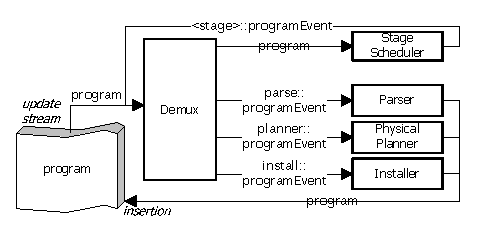
\includegraphics{visio/DefaultCompiler}
\caption{The cyclic dataflow of Evita Raced, showing only the default compilation stages.}
\label{fig:basecompiler}
\end{center}
\end{figure}

The StageScheduler and any compilation stages (whether built-in or
runtime-installed) are interconnected via the simple dataflow
illustrated in Figure~\ref{fig:basecompiler}. This is the same dataflow
that P2 constructs for all Overlog programs. It consists of a C++ ``demultiplexer'' that
routes tuples from its input (on the left) to individual event handlers listening for
particular tuple names (the arrows leaving the Demux element in the
figure contain the name of the tuple for which the four components to the
right listen).  We have not changed P2's dataflow architecture~\cite{loo-sosp05}, and its
details are not required for the rest of this paper.  

Consider the simplicity of this approach as compared to the explicit
stage-wiring  sketched above. When a new compilation stage is installed
at runtime, the Installer (Section~\ref{sec:installer})
simply connects it to the {\em Demux} element, listening for
\ol{<stage>::programEvent} tuples, before updating the corresponding
tuple in the \ol{program} table. 
Then the StageScheduler who receives the updated \ol{program} tuple uses
the value of its $depends$ attribute  to insert appropriate 
\ol{StageLattice} tuples into the corresponding table of the
system catalog. Subsequent \ol{program} tuples being compiled will be directed to
the newly installed compiler stage by the StageScheduler as the updated
\ol{StageLattice} dictates.

To sum up, the life cycle of a program compilation starts when a user
submits a \ol{program} tuple to the system with a \ol{null} stage
attribute. The StageScheduler receives that \ol{program} tuple and
generates a
\ol{parse::programEvent} tuple (the Parser being the source stage in the
lattice), which is routed by the Demux element to
the Parser stage. When the Parser is done, it updates that \ol{program} tuple
in the corresponding table, changing the tuple's attribute to
``Parser.''  The StageScheduler receives the \ol{program} tuple, and routes a
\ol{planner::programEvent} to the Demux and eventually the Physical Planner, which goes round the loop again to the
Installer.  Finally, once the Installer is done and notifies the
StageScheduler via a \ol{program} tuple with the \ol{stage} attribute set to
``Installer,'' the StageScheduler concludes the compilation process.
If the Overlog program being parsed is itself a new compilation stage, then after
installation, the scheduler updates the stage lattice.


\subsection{Compiler Bootstrapping}
\label{sec:bootstrap}
The previous architectural discussion neatly sidestepped a natural question: how is an Evita Raced compiler containing many Overlog stages bootstrapped, so that it can compile its own Overlog specification?
As in many metaprogramming settings, this is done by writing a small bootstrap  in a lower-level language. Evita Raced is initialized by a small C++ library that constructs the cyclic dataflow of Figure~\ref{fig:basecompiler}, including the three default stages shown, which are themselves written in C++. %The entire bootstrap, including the stages is {\bf XXX} lines of C++ (and a).  
Together, this code is sufficient
to compile simplified Overlog (local rules only, no optimizations) into
operational P2 dataflows. We next describe each of these stages in a bit
more detail, since they form the foundation of the Evita Raced runtime.


% \jmh{This paragraph was saved from a conflict with Tyson's checkin.  Joe will merge it in Tuesday night.
% The {\em stage scheduler} is a dataflow element that is responsible for providing the inputs to a 
% stage and processing any outputs from a stage. The input to a stage module is a tuple containing the 
% identifier of the program that it is responsible for
% processing. When the stage completes its task is will insert a new program tuple into
% the \ol{program} table with an updated $state$ attribute value that indicates (to the scheduler) the completion 
% of the stage operation on the input program. The program insertion triggers a new
% \ol{programEvent} tuple that is again directed to the stage scheduler, and the process repeats with
% the next scheduled stage in the compilation order. Stage execution order is determined by
% a relation of stage dependencies. The stage scheduler schedules
% a stage based on the dependency graph relation installed by the bootstrap process and the current 
% value of the $state$ attribute in the program tuple. The process completes when the program $state$ 
% attribute reaches stage that no other stage depends on.
% }


% \subsubsection{Default Query Compilation}
% 
% Figure~\ref{fig:basecompiler} shows a dataflow perspective of our default
% metacompiler. A user submits a new program to the system by inserting a tuple into the \ol{program} table.
% The program tuple contains initial values for all the attributes in the program table (see Table~\ref{tbl:tables}). 
% A program table insertion triggers a \ol{programEvent} event tuple that contains the program 
% identifier attribute value.  The "Demux" dataflow element routes the \ol{programEvent} tuple to the
% stage scheduler element, which determines the order in which a stages execute on the input
% program. 
% \petros{The job of the scheduler is a bit nebulous. Is there something
% you can say here to make clear what that does?}
% 
% 
% The input to a stage module is a tuple containing the identifier of the program that it is responsible for
% processing. When the stage completes its task is will insert a new program tuple into
% the \ol{program} table with an updated $State$ attribute value that indicates (to the scheduler) the completion 
% of the stage operation on the input program. The program insertion triggers a new
% \ol{programEvent} tuple that is directed to the stage scheduler, and the process repeats with
% the next scheduled stage in the compilation order. Stage execution order is determined by
% a relation of stage dependencies. The stage scheduler schedules
% a stage based on the dependency graph and the current value of the $State$ attribute in the program tuple. 
% The process completes when the program $State$ attribute reaches stage that no further stage depend on.
% 
\subsubsection{Parser}

The Parser passes the program text it receives in the \ol{programEvent}
through a traditional lexer/parser library specified using
flex~\cite{flexUrl} and bison\cite{bisonUrl}; this library code returns
a standard {\em abstract syntax tree} representation of the text.
Assuming the Parser does not raise an exception due to a syntax error,
it walks the abstract syntax tree, generating Metacompiler Catalog
tuples for each of the semantic elements of the tree. In addition to
recognizing the different terms of each rule, the parser also annotates
each term with its position in the given program.  By convention, the
first term of a rule body is the event predicate of the rule, if one
exists.  By the same convention, the term in the last position for a
rule is the head predicate.



\subsubsection{Physical Planner}
\label{sec:planner}

The Physical Planner stage is responsible for doing a na\"{i}ve
translation of Metacompiler Catalog tuples (i.e., a parsed Overlog program) into a dataflow program. It essentially takes each rule and deterministically translates it into a dataflow graph language, based on the positions of terms in the rule.

More specifically, for each rule the Planner considers each term
(predicate, selection or assignment) in order of position attribute.
The predicate representing the event stream is always planned first,
and registers a listener in the Demux element (recall
Figure~\ref{fig:basecompiler}).  The terms following the event stream
are translated, left-to-right, into a C++ dataflow in the same way that
the original P2 system did, so we do not address them further here.

We do mention three specific details. First, whereas the original P2
system translated a logical query plan directly to a software dataflow
structure in C++, we have chosen to create an intermediate, textual
representation of the dataflow. This representation is in a language
akin to the Click router's dataflow language, but we omit its details here. 

Second, unlike the original P2
system, we have introduced a number of access methods for in-memory
tables. Our \ol{predicate} relation contains the access method as one of
the attributes, and we have modified the P2 physical planner to choose
the appropriate dataflow element that implements the given access
method. 

%% Those are naturally introduced to the P2 physical planner
%% machinery and otherwise
%% creates
%% a listening port in the P2 {\em Demux} on the event stream name. The predicates mentioned in the rule that
%% do not represent the event stream represent lookup operations (joins) on the referenced base relation.
%% A join operator is planned for a predicate by taking the input stream and schema and joining 
%% it - using the $access\_method$ given by the \ol{predicate} tuple - with a base relation producing a new tuple 
%% stream with the join schema. 
%% A selection term plans a filter operator that applies the $boolean$ attribute value to the input 
%% stream and passes only tuples that satisfy this expression to the output stream. \jmh{Again the "plans an operators that does X" doesn't mean much to me.}An assignment term 
%% plans a assignment operator that uses the input stream to evaluate the $value$ attribute (in the \ol{Assign}
%% tuple) to an atomic value. If the input stream contains an attribute named by $variable$ 
%% (in the \ol{Assign} tuple) then the value of that attribute is substituted in the input
%% stream, otherwise a new attribute is added to the input schema with the given value 
%% in the output stream. After all rule body terms have been planned, the planner adds a projection operator
%% that projects the output tuple stream onto the head predicate.

% generates a physical plan for each rule in a program. The execution order of a physical plan in 
% P2 is a leaf-to-root path, with the leaf corresponding to the event predicate and the root being the head 
% predicate. All predicates that lie in between the leaf and the root path are joined against the respective 
% base relation according to the access method given by the predicate tuple. 
% \petros{I would go as far as saying that the physical plan you derive is
% expressed in an operator language reminiscent of the Click
% language. Since we concentrate on logical plan manipulations here we
% don't go into details. The important thing to point out is that whatever
% you do is not tied to a particular runtime; one could take this physical
% plan and install it on a different runtime that isn't our dataflow but
% something else.}

% The initial operator is always the event predicate and it determines when the rule should fire. 
% If the rule does not contain an event predicate then a delta rewrite must be preformed on the rule. 
% The delta rewrite converts the original rule into a set of new rules
% that trigger whenever a side affect\petros{``side affect'' should be
%   ``side effect'' everywhere.} 
% occurs on a table predicate mentioned in the original rule. The delta rewrite is presented 
% in~\cite{boonSigmod}, and we fully adopt this rewrite in our metacompiler. The position attribute 
% defined by each predicate tuple determines the position of the corresponding physical operator in 
% the physical plan. Select and assign operators are also planned at the position indicated by the 
% respective table tuple.

Third, as mentioned before, Overlog rules may have no event predicate
(e.g., ``\ol{table1 :- table2, table3.}''). 
The physical planner converts such rules to (multiple) event rules via the {\em delta
rewrite} of Loo, et al.~\cite{loo-sigmod06}. (E.g., ``\ol{table1 :- delta\_table2,
table3.}'' and ``\ol{table1 :- table2,
delta\_table3.}''.) As in~\cite{loo-sigmod06} \ol{delta\_table} denotes a stream conveying
insertions, deletions, or timeout refreshes to tuples of the table
\ol{table}.


\subsubsection{Plan Installer}
\label{sec:installer}

Given the output of the Physical Planner in the dataflow specification
language, what remains is to parse the
textual representation of the dataflow,  construct the
corresponding C++ elements, and ``wire them up'' accordingly. We have
implemented this 
``physical plan compiler'' in C++, and housed it within the
Installer stage.  Once these elements and their connections are
instantiated, the Plan Installer stage stitches them into the P2
runtime's overall dataflow graph, as described in~\cite{loo-sosp05}.
As noted in~\ref{sec:metaarch}, this infrastructure made it easy for us to extend P2 with the ability to modify its dataflow graph at runtime,
a feature not available in the released system. 
% Since our focus here
% is on plan optimization, we omit the engineering
% details of that contribution.
% 

\subsection{Discussion}
The metacompilation approach of Evita Raced led us to naturally design the system extensibility around issues of data storage and dataflow, rather than library loading and control flow modifications.  While any rule-based system is easier to extend than a procedural system, the internal implementation of Evita Raced is especially elegant, due to our thorough embrace of the native dataflow infrastructure, which we use both to execute optimization code, and orchestrate stages via precedence tables and the StageScheduler cycle.  The result of this design is that
even a major addition to the Evita Raced compiler entails very minimal
modification to the runtime state: only the addition of a pair of
dataflow edges to connect up the new stage, and the insertion of
precedence tuples in a single table.  Beyond the StageScheduler and the three bootstrap stages, no additional extensibility code was added to P2 to support Evita Raced.

Despite its simplicity, Evita Raced is flexible enough that we have used it to enhance P2 with support for new languages at both its input and output.  First, by extending the Parser element and registering some Overlog rules, we have been able to get P2  to optimize and rewrite programs written in a new language, which extends Overlog with the ability to attest to the provenance of data in a manner similar to that of~\cite{abadi-netdb07}.  Second, we have been able to use Evita Raced to cross-compile Overlog programs into dataflow specifications that execute on the DSN platform, a declarative networking system that runs on wireless sensor nodes~\cite{chu-sensys07}.
%  In Section~\ref{sec:dsn} we present results from running Evita Raced plans in DSN on Berkeley Mote hardware.  


\section{Query Compilation Stages}
\label{sec:rewrite}
% \jmh{This paragraph is thoroughly redundant with hte previous section and can be chopped.  However, it'd be nice to have some kinda warmup text here.}
% A compilation stage written in the P2 query language is dynamically installed into the compiler 
% at runtime, using the same compilation path taken by any Overlog program. The stage programmer 
% inserts a program tuple containing the text of an Overlog program. The programmer also specifies, 
% in the {\em depends} attribute of the program tuple, a single stage that should execute immediately 
% before the installed stage.  After the insertion into the program table, the stage scheduler receives 
% the \ol{programEvent} tuple, which it uses to access the program tuple. The program is processed
% by the stages that appear in the current dependency graph relation. The stages treat the program 
% no differently than any other program. Once the program has been successfully installed, the stage 
% scheduler will then notice that the $depends$ attribute of the program tuple contains a 
% reference to a preexisting stage. 
% The dependency reference informs the stage scheduler that installed program represents a new stage, and 
% that it should update the dependency relation accordingly. After performing the update to the dependency
% relation, the new stage will be included in the compilation process of future input programs. 

Having described the Evita Raced infrastructure, we now turn our
attention to the issue of specifying query optimizations in Overlog.  In
this section we  describe three of the compiler stages we have developed
for Evita Raced. 
Section~\ref{sec:systemr} discusses a dynamic programming optimizer stage akin to that of
System R. Section~\ref{sec:magic} describes a stage that performs 
magic-sets rewrite on recursive Overlog programs.
Finally, Section~\ref{sec:localization} describes our
reimplementation in Evita Raced of localization  from Loo et
al.~\cite{loo-sigmod06}. 

\subsection{System R Optimization}
\label{sec:systemr}

The System R optimizer paper by Selinger, et al. is the canonical textbook framework for database query optimization~\cite{selinger}.  The paper laid out for
the first time the notion that query optimization can be decomposed
into two basic parts: query plan cost
estimation and plan enumeration.  While this algorithm is traditionally implemented inside
the heart of a database system via a traditional procedural
programming language, both of these tasks are
naturally specified in a declarative query language.  To perform cost
estimation, System~R requires data statistics like relation
cardinalities and index selectivities; Overlog is a fitting language to
collect these statistics, especially in a distributed fashion over all
relation partitions. In our description we omit statistics gathering.

We focus instead on the basic dynamic programming algorithm for the
state-space enumeration at the heart of the System R optimizer.  This
algorithm enumerates query plans for increasingly-large subgoals of the
query optimizer.  It fills in a dynamic programming table keyed by the
plan identifier.  The dynamic programming task is
to fill in this table with the lowest-estimated-cost query plan among
all plans producing an {\em equivalent} output relation (i.e., plans
composed of the same terms).  
In the System R optimizer, the {\em principle of
optimality} is assumed to hold: the lowest-cost solution to some
plan will be built from the optimal solutions to subplans.  Thus dynamic
programming can proceed in ``bottom-up'' fashion.  Each rule's event
predicate is the ``outermost,'' streaming relation in a query plan for the rule.  For a given rule,
the optimizer generates plans of size $k$ terms by appending a single
(thus unused)
term from the rule body to the optimal plan of
size $k-1$ terms.

% An
% aggregation query chooses optimal plans from the set of equivalent plans.
We first describe the rules for plan generation and conclude with the
rules for optimal plan selection.

\subsubsection{Plan Generation}
\label{sec:plangen}

\begin{figure}
\centering
\begin{boxedminipage}{\linewidth}
\scriptsize{\tt
pg1 {\small \bf plan}(@A, Pid, Rid, PlanID, SubPlanID, Type, TypeID, \\
\datalogspace \xspace Plan, Schema, Card, Cost, Pos, AM, Sort, TermC) :- \\
\datalogspace {\small \bf systemr::programEvent}(@A, Pid, \_, \_, \_, \_, \_, \_),\\
\datalogspace {\small \bf rule}(@A, Rid, Pid, \_, \_, \_, \_, TermC),\\
\datalogspace {\small \bf predicate}(@A, PredID, Rid, \_, \_, \_, \_, \\
\datalogspace \datalogspace \datalogspace Schema, Pos, \_, \_),\\
\datalogspace Pos == $1$,\\
\datalogspace PlanID := {\em f\_idgen()}, SubPlanID := $null$,\\
\datalogspace Type := "Predicate", TypeID := PredID,\\
\datalogspace Plan := {\em f\_cons}(PredID, $null$),\\
\datalogspace Card := $1$, Cost := $1$,\\
\datalogspace AM := "STREAM", Sort := $null$.
}
\caption{\label{fig:planseed}Plan seed rule.}
\end{boxedminipage}
\end{figure}

Figure~\ref{fig:planseed} shows the optimizer rule  that creates
the initial plan for each rule from the event predicate. The \ol{plan} tuple
contains a query plan for a given rule, and the plan's \ol{size} reflects the number of
term identifiers in the $Plan$ attribute (i.e., the number of leaves in the plan tree). The optimizer listens on the \ol{programEvent} event stream in
rule \ol{pg1}, which will start the optimization process.  
The \ol{programEvent} tuple is subsequently joined with the \ol{rule} table along the 
$Pid$ (program identifier) attribute to obtain the set of rules defined in the input program. 
The resulting set of rule tuples are each joined with the \ol{predicate} table along the 
$Rid$ (rule identifier) attribute. The result of this join produces a tuple for each predicate term 
defined by a given rule. The predicate term assigned to position~$1$ ($Pos == 1$) is
by convention the event predicate term.  For each 
event \ol{predicate} tuple in each rule of the input program, rule \ol{pg1} adds a new 
plan to the \ol{plan} table. The $Plan$ attribute represents the initial plan list,
starting with the term identifier ($PredID$) that identifies streaming predicates.
Plan generation proceeds by appending term identifiers to this list when
constructing new plans from optimal subplans.

The optimizer defines a set of plan generation rules that extend the
best plan found with $k$ terms with a new thus far unused term from the
rule body. Each such rule joins the \ol{bestPlanUpdate} event predicate
(generated when a new $k$-term plan is found) with unused terms in the
rule. If the new term considered is a predicate, then the new plan
must define an access method
that identifies the physical join operator, which
takes the optimal subplan and ``joins it'' with the predicate table. The access methods we presently 
support are scanned and index-nested-loop-join, as well as merge-join. 
The rules for plan generation from rule predicates are defined around the supported access methods. 
Due to space constraints, we only show the rules that generate plans for nested-loop-join 
and index nested-loop-join access methods.\footnote{A complete description of our rules 
in an extended technical report is available to the conference chair
during double blind reviewing.}

\begin{figure}
\centering
\begin{boxedminipage}{\linewidth}
\scriptsize{\tt
pg2 {\small \bf plan}(@A, Pid, Rid, {\em f\_idgen()}, PlanID, "Predicate", PredID, \\
\datalogspace \xspace Plan, Schema, Card, Cost, \\
\datalogspace \xspace OuterPos+$1$, AM, $null$, TermC) :-\\
\datalogspace {\small \bf bestPlanUpdate}(@A, Pid, Rid, PlanID),\\
\datalogspace {\small \bf plan}(@A, Pid, Rid, PlanID, \_, \_, \_, OuterPlan, \\
\datalogspace \xspace \xspace OuterSchema, OuterCard, OuterCost, OuterPos, \\
\datalogspace \xspace \xspace \_, \_),  \\   
\datalogspace {\small \bf predicate}(@A, PredID, Rid, \_, \_, Tid, \_, \\
\datalogspace \xspace \xspace PredSchema, PredPos, \_, \_),\\
\datalogspace PredPos < TermC,\\
\datalogspace {\small \bf table}(@A, Tid, \_, \_, \_, \_, TCard, \_),\\
\datalogspace {\em f\_contains}(PredID, OuterPlan) == $false$,\\
\datalogspace Card := OuterCard * TCard / $10$,\\
\datalogspace Cost := OuterCost + (OuterCard * TCard),\\
\datalogspace AM := {\em f\_cons}("SCAN", $null$), \\
\datalogspace Plan := {\em f\_cons}(PredID, OuterPlan), \\
\datalogspace Schema := {\em f\_merge}(OuterSchema, PredSchema).\\
\\
pgn {\small \bf planUpdate}(@A, Pid, Rid, PlanID, SubPlanID, Sort) :- \\
\datalogspace {\small \bf plan}(@A, Pid, Rid, PlanID, SubPlanID, \_, \_, \\
\datalogspace \xspace \xspace \_, \_, \_, \_, \_, \_, Sort, \_).
}
\caption{\label{fig:plangen1}Scan-join access method.}
\end{boxedminipage}
\end{figure}

A nested-loop-join plan access method is generated for any table predicate appearing
in the rule body. Rule \ol{pg2} in Figure~\ref{fig:plangen1} generates a
(scanned) nested-loop-join 
plan on all rule body table predicates not mentioned in the $OuterPlan$ attribute of the \ol{plan}
predicate representing the subplan. The \ol{plan} tuple representing the subplan is joined with 
the \ol{predicate} (all predicate terms in the rule body) table followed by another join with 
the \ol{table} (all tables in the system) table. The result of these join operations produce all 
term predicates mentioned in the rule that have a matching table identifier definition. 
The selection predicate $PredPos < TermC$ ensures that we do not
consider the rule head predicate (last in the rule's terms by
convention). The function $f\_contains$ tests for containment of the predicate in the subplan (outer plan). 
Any tuples that meet the constraints imposed by this rule generate a new \ol{plan} 
tuple with the ``SCAN'' access method (since the predicate table will be scanned for each outer tuple). 
Each new plan tuple is given a new $Plan$ attribute that appends the $PredID$ to the $OuterPlan$ 
subplan attribute. 
The cardinality ($Card$) and cost ($Cost$) estimates are given values based on some costing 
measure, which in this case makes use of best plan cardinality and cost estimates, and the predicate 
table cardinality.

\begin{figure}
\centering
\begin{boxedminipage}{\linewidth}
\scriptsize{\tt
pg3 {\small \bf plan}(@A, ...) :-\\
\datalogspace ...\\
\datalogspace {\small \bf table}(@A, Tid, Tablename, \_, \_, \_, TCard, \_),\\
\datalogspace {\small \bf index}(@A,Iid,Tablename,Key,Type,Selectivity),\\
\datalogspace {\em f\_contains}(PredID, OuterPlan) == $false$,\\
\datalogspace {\em f\_indexMatch}(OuterSchema, PredSchema, Key),\\
\datalogspace Card   := OuterCard * (Selectivity * TCard),\\
\datalogspace Cost   := OuterCost + Card,\\
\datalogspace AM := {\em f\_cons}(Type, Iid),\\
\datalogspace ...
}
\caption{\label{fig:plangen2}Index-join access method (diff from Figure~\ref{fig:plangen1}).}
\end{boxedminipage}
\end{figure}

An index-nested-loop-join plan is generated by rule \ol{pg3} in Figure~\ref{fig:plangen2}. The main
difference between this rule and rule \ol{pg2} is the additional \ol{index} predicate, which
adds index definitions to the resulting table predicate tuples. The function {\em f\_indexMatch}
tests if the index can be used to perform the join using attributes from the best plan schema ($OuterSchema$)
and attributes from the predicate table ($PredSchema$). Any tuple results from this plan are assigned 
cardinality and cost estimates based on some cost function, which uses the additional index selectivity
information given by the $Selectivity$ \ol{index} predicate attribute.
We also support range predicates in our index-nested-loop-joins but do
not show the 3 relevant rules here.

A merge-join performs a join of a plan with a table predicate mentioned in the rule body along
some sorting attribute. The tuple set from the outer plan and the predicate table must
be ordered by the sorting attribute. The output of a merge-join operation preserves
the sorting attribute order. Therefore, the \ol{plan} predicate generated by the merge-join rule 
includes the sorting attribute in the value of the $Sort$ \ol{plan} predicate. We note that the $Sort$
attribute in the \ol{table} plan table identifies the sorting attribute of the table.
A $null$ valued $Sort$ attribute, in either the outer relation \ol{plan} predicate or the inner relation
\ol{table} predicate, means that the relation is unordered, and must be presorted prior to the merge-join operator.  
The cost of a merge-join operator depends on need to presort either relation. 

\subsubsection{Best plan selection}
\label{sec:bestplan}

\begin{figure}
\centering
\begin{boxedminipage}{\linewidth}
\scriptsize{\tt
bp1 {\small \bf bestCostPlan}(@A, Pid, Rid, Plan1, Sort1, {\small \bf a\_min}<Cost>) :- \\
\datalogspace {\small \bf planUpdate}(@A, Pid, Rid, \_, Plan1, Sort1), \\
\datalogspace {\small \bf plan}(@A, Pid, Rid, \_, \_, \_, \_, \\
\datalogspace  \xspace \xspace \xspace Plan2, \_, \_, Cost, \_, \_, Sort2, \_), \\
\datalogspace {\em f\_setequals}(Plan1, Plan2), Sort1 == Sort2. \\
\\            
bp2 {\small \bf bestPlan}(@A, Pid, Rid, PlanID, Plan2, Cost) :- \\
\datalogspace {\small \bf bestCostPlan}(@A, Pid, Rid, Plan1, Sort1, Cost), \\
\datalogspace {\small \bf plan}(@A, Pid, Rid, PlanID, \_, \_, \_, \\
\datalogspace \xspace \xspace \xspace Plan2, \_, \_, Cost, \_, \_, Sort2, \_), \\
\datalogspace {\em f\_setequals}(Plan1, Plan2), Sort1 == Sort2.\\
\\            
bp3 {\small \bf bestPlanUpdate}(@A, Pid, Rid, PlanID) :- \\
\datalogspace {\small \bf bestPlan}(@A, Pid, Rid, PlanID, \_, \_).
}
\caption{\label{fig:bestplan}Best plan selection.}
\end{boxedminipage}
\end{figure}

Figure~\ref{fig:bestplan} shows two rules that select the best plan from a 
set of equivalent plans, in terms of the output result set and the ordering 
properties of the result set. The \ol{bestCostPlan} predicate picks the
plan with the minimum cost from the set of equivalent plans. This aggregation 
query groups along the program identifier, rule identifier, plan list, and sort
attribute. The function {\em f\_setequals} tests whether the set of term identifiers in the two argument plans are the same, regardless of the order. The inclusion
of the sort attribute in the group condition ensures the handling of what Selinger calls ``interesting orders''~\cite{selinger}, along with optimal subplans.
 
The aggregation rule \ol{bp1} triggers whenever a new plan is added to the \ol{plan} 
table (indicated by the \ol{planUpdate} event). Then, the \ol{bestCostPlan} predicate is used 
in rule \ol{bp2} to select the identifier of the best plan, which is inserted into the \ol{bestPlan} 
table. An update to the \ol{bestPlan} table triggers a new \ol{bestPlanUpdate} event that the 
plan generation rules, described in Section~\ref{sec:plangen}, use to build new candidate plans.

\subsection{Magic-Sets Rewrite}
\label{sec:magic}

The magic-sets rewrite is an optimization that can reduce the amount 
of computation in recursive Datalog queries. It combines the
benefits of top-down and bottom-up evaluation of logic,
without the disadvantages of either~\cite{ullmanNotes}. 

Datalog-oriented systems like P2 perform a bottom-up (\emph{forward chaining}) evaluation 
on each rule, starting with known facts (tuples), and recursively
resolving body predicates to the head predicate. The advantage of this strategy is
that the evaluation is data driven (from known facts to possible
deductions) and will not enter infinite loops for some statically
verifiable \emph{safe} programs. 
For example, consider again a snippet of the shortest path program, in
Figure~\ref{fig:querySP}. The query asks for the shortest
path from all nodes to node ``localhost:10000''. A bottom-up evaluation
applies the \ol{link} tuples to rule \ol{r1}, creating initial {\tt
path} tuples. Those are \ol{path} tuples until it reaches a
fixed-point.  Any \ol{path} tuples matching
``localhost:10000'' on their second attribute match the programmer's query.

Bottom-up evaluation generates some \ol{path} tuples that do not have
``localhost:10000'' in the second attribute and therefore cannot satisfy
the programmer's query.  In contrast, top-down
(\emph{backward chaining}) evaluation (e.g., in the Prolog language), starts with the query
predicates as the top-level goals, and recursively identifies rules
whose head predicates unify with needed goals, replacing them with the
subgoal predicates in the rule body, until all subgoals are satisfied by
known facts or rejected when no further recursion is possible. The
advantage of a top-down evaluation strategy is that it avoids resolving
goals that are not needed by the posed queries.  In the example, a top-down
evaluation unifies the query
predicate with the head predicate of rules \ol{r1} and
\ol{r2}\footnote{In P2 the location attribute of a query rule is always
bound to the local node identifier.}.  Therefore, the \ol{path}
predicate unification binds the $@X$ attribute to the current node
identifier and the $Y$ attribute to ``localhost:10000'' in both rules,
which is carried over to the predicates in the rule body. The binding of
$@X$ and $Y$ attributes in rules \ol{r1} and \ol{r2} means that these
rules will only look for tuples of the form
$path(LOCALHOST,"localhost:10000",P,C)$ as well as tuples that can help form
such \ol{path} tuples, but nothing else~\footnote{A
detail of the SPMD networked nature of Evita Race is that queries run
everywhere imply a binding for the location specifier attribute to the
local host's address, conveyed by the \ol{LOCALHOST} macro, hence the
contents of query tuple.}.


\begin{figure}[!t]
\centering
\begin{boxedminipage}{\linewidth}
\scriptsize{\tt
link(@"localhost:10000", "localhost:10001").\\
link(@"localhost:10001", "localhost:10002").\\
...\\
\\
r1 path(@X,Y,P,C) :- \\
\datalogspace link(@X,Y,C), P := f\_cons(X,Y). \\
\\
r2 path(@X,Y,P,C) :- \\
\datalogspace link(@X,Z,C1), path(@Z,Y,P2,C2),\\
\datalogspace f\_contains(X,P2) == false, \\
\datalogspace P := f\_cons(X,P2), C := C1 + C2. \\
\\
Query: path(@LOCALHOST,"localhost:10000",P,C).
}
\caption{\label{fig:querySP}Relevant rules from Figure~\ref{fig:overlogSP}.}
\end{boxedminipage}
\end{figure}

Ullman's magic sets algorithm operates in three phases: program analysis,
program rewrite, and filter population.
\begin{figure}[!t]
\begin{center}
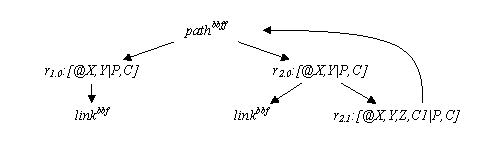
\includegraphics{visio/RuleGoalGraph}
\caption{Rule/Goal graph of the program in Figure~\ref{fig:querySP}.}
\label{fig:rggraph}
\end{center}
\end{figure}


Magic-sets algorithms add extra selection predicates to the rules of a program to
emulate the goal-oriented execution of top-down evaluation (this is
sometimes called \emph{sideways information passing} or
SIP). Conceptually, given a rule of the form
\[
H_p \ \text{\ol{:-}}\  G_1, G_2, ..., G_k
\]
where $H_p$ is the head predicate $p$ and $G_{1,...,k}$ are the goal
predicates in the order of appearance in the rule, a magic-sets
algorithm intersperses selection predicates $s_{1,...,k}$ to generate rule
\[
H_p \ \text{\ol{:-}}\  s_1, G_1, s_2, G_2, ..., s_{k}, G_k
\]
Facts for the magic predicates are generated according to bindings of
the attributes of $H_p$ in the user's query, or other identified
attribute bindings in the program. In Evita Raced we create a magic-sets
optimization that implements the description given in Ullman's course notes~\cite{ullmanNotes}. 
A very brief overview by example follows.



\subsubsection{Magic-sets By Example}

In the program analysis phase, the algorithm traverses every rule,
starting with those whose rule heads that match the query predicate, to build
a recursive tree structure called the {\em Rule/Goal} graph. This graph
consists of \emph{rule} and \emph{goal} vertices.  A goal
vertex consists of a predicate with an
adornment indicating which of the attributes in the predicate
are bound and which free.  A rule vertex represents the bound/free state of
all seen variables within a rule body, up to a particular position in its
left-to-right execution. A rule with $k$ body predicates will
result in exactly $k$ rule vertices corresponding to its positions
$[0,...,k-1]$.

Figure~\ref{fig:rggraph} illustrates the full graph for our example.  To
build the graph, the algorithm starts with a goal predicate (at first,
the query predicate---\ol{path} in our example), and creates a goal
vertex in the graph with the appropriate adornment ($\mathit{bbff}$ for
\ol{path} since the query binds its first two variables). For every
rule with that goal predicate as its head, the algorithm traverses the
rule body from left to right, creating a child rule vertex for every
$0$-th position variable binding.  For rule \ol{r2} in the example, the
rule vertex for position $0$ ($r_{2,0}$) has variable state $[X,Y|P,C]$,
which denotes that variables \ol{X,Y} are bound (to the same values as
those ``pushed down'' from the goal vertex) and \ol{P,C} are free.
Given a rule vertex for position $i$, two children are created: a goal
vertex for the next predicate after position $i$ and a rule vertex for
the next position in the rule (unless the body's end has been reached).
In the running example, the child goal vertex corresponds to the {\tt
link} predicate that appears at position $0$, with adornment
$\mathit{bff}$ since \ol{X} is already bound at this point in the
evaluation, but \ol{Z, C1} are not.  Similarly, the child rule vertex
at position $1$ contains the variable signature $[X,Y,Z,C1|P,C]$ since
\ol{link} added some bound variables.  The process continues until all
rule and goal vertices have been constructed and connected; 
only a single goal vertex can exist with the same predicate and
adornment, as is the case for the \ol{path} vertex with adornment
$\mathit{bbff}$.   It is easy to see how the rest
of the rule/goal graph is constructed. After all vertices have been
generated given the chosen rules, any predicates with a unique adornment
in the graph are added to the goals and the rules producing them are
recursively traversed.


In the program rewrite phase, Ullman's algorithm traverses the rule/goal
  graph generating magic predicates for each ``goal'' vertex that is
  unique for its (IDB) predicate; in the example, there are multiple vertices
  with different adornments for \ol{link}, but only one for \ol{path},
  so only \ol{path} is chosen.  This magic predicate is inserted in
  the $0$-th position of all rules with the corresponding goal predicate
  as the rule head, with the bound variables of the signature as
  attributes. In the example, the magic predicate for \ol{path} has the
  form \ol{magic\_path(@X, Y)} since \ol{X, Y} are the bound
  variables in the signature of the ``goal'' vertex.  Also
  \emph{supplementary} predicates are similarly created for all
  encountered ``rule'' vertices during the graph traversal and inserted
  within the corresponding original rule.  For example, {\tt
  sup\_r2\_1(@X,Y,Z,C1)} 
  is created for ``rule'' vertex $r_{2,1}$ with the bound variables of
  the adornments in the vertex, and placed in the original rule \ol{r2}
  between the \ol{link} and \ol{path} predicates.


\begin{figure}[!t]
\begin{boxedminipage}{\linewidth}
\scriptsize{\tt
link(@"localhost:10000", "localhost:10001").\\
link(@"localhost:10001", "localhost:10002").\\
...\\
magic\_path(@LOCALHOST, "localhost:10000"). \\
\\
r1\_g3a path(@X, Y, P, C) :- \\
\datalogspace magic\_path(@X,Y), link(@X,Y,C), P := f\_cons(X,Y).\\
\\
r2\_g1a magic\_path(@X, Y) :- \\
\datalogspace sup\_r2\_1(@X, Y, Z, C1). \\
\\
r2\_g3a sup\_r2\_1(@X, Y, Z, C1) :- \\
\datalogspace magic\_path(@X, Y), link(@X, Z, C1). \\
\\
r2\_g3c path(@X, Y, P, C) :- \\
\datalogspace sup\_r2\_1(@X, Y, Z, C1), path(@Z, Y, P2, C2). \\
\datalogspace f\_contains(X, P2) == false, \\
\datalogspace P := f\_cons(X, P2), C := C1 + C2. \\
\\
Query: path(@LOCALHOST,"localhost:10000",P,C).
}
\caption{\label{fig:magicSP}A magic-sets rewrite of
      the rules in Figure~\ref{fig:querySP} (materialize statements not shown).}
\end{boxedminipage}
\end{figure}

Finally, in the filter population phase, the algorithm maintains the
magic predicate relation, which was placed within the rewritten program
in the previous phases.  Any a priori known bindings about the root goal vertex
(e.g., from the user's query) are 
placed in the magic relation. In the example, the fact ``\ol{magic\_path(LOCALHOST, "localhost:10000").}'' is put into the
database from the bindings in the \ol{path} query.  Also, any edges in
the rule/goal graph that start from a rule vertex and end at a goal vertex, with a
unique adornment (i.e., upward arrows in the recursive tree that constitutes the graph), are written as
rules that generate new magic tuples from new tuples of the rule
node's supplementary predicate. In the example, rule \ol{r2\_g1a}~\footnote{Rule names that
deal with magic and supplementary predicate maintenance were named according
to Ullman's rule groups. For instance, rules named \ol{r*\_g3[a-c]} follow rule group 3
and rule \ol{r2\_g1a} follows rule group 1.}  adds
more magic facts as more \ol{sup\_r2\_1} tuples are produced.

Our rewrite implementation of this algorithm first traverses every rule
from head predicate to body predicates from left to right, constructing
the rule/goal graph in the recursive manner of the program analysis, in
a single fixpoint.  Then the new program rules (and replacement of old
rules) for the program rewrite and filter population phases are
performed via a traversal of the newly constructed rule/goal graph in a
subsequent fixpoint. Finally, initial magic facts are created by direct
translation from the query.  Other details we elide here for brevity
involve detecting eligibility of a predicate for a magic-sets rewrite
(whether or not it has a unique adornment in the rule/goal graph), state
cleanup, etc. 

\begin{figure}[t]
\begin{boxedminipage}{\linewidth}
\scriptsize{\tt
materialize(sup,infinity,infinity,keys(2,3,4)). \\
materialize(adornment,infinity,infinity,keys(2,5,6)). \\
materialize(idbPredicate,infinity,infinity,keys(2,3)). \\
\\
mg1 {\small \bf goalCount}(@A, Pid, PredName, {\small \bf a\_count}<*>) :- \\
\datalogspace {\small \bf idbPredicate}(@A, Pid, PredName), \\
\datalogspace {\small \bf adornment}(@A, Pid, Rid, Pos, PredName, Sig). \\
\\
mg2 {\small \bf magicPred}(@A, Pid, GoalName, Sig) :- \\
\datalogspace {\small \bf goalCount}(@A, Pid, GoalName, Count), \\
\datalogspace {\small \bf adornment}(@A, Pid, \_, \_, GoalName, Sig). \\
\datalogspace Count == 1. \\
\\
mg3 {\small \bf sup}(@A, Pid, Rid, Pos, Name, Schema) :- \\
\datalogspace {\small \bf magicPred}(@A, Pid, Name, Sig), \\
\datalogspace {\small \bf rule}(@A, Rid, Pid, \_, HeadPid, \_, \_, \_), \\
\datalogspace {\small \bf predicate}(@A, HeadPid, Rid, \_, Name, \_, \_, Schema, \\
\datalogspace \datalogspace \_, \_, \_), \\
\datalogspace Schema := {\em f\_project}(Sig, Schema), \\
\datalogspace Name := "magic\_" + Name, Pos := 0. \\
\\
mg4 {\small \bf supNext}(@A, Pid, Rid, Pos+1, Schema) :- \\
\datalogspace {\small \bf sup}(@A, Pid, Rid, Pos, Name, Schema). \\
\\
mg5 {\small \bf sup}(@A, Pid, Rid, Pos, Name, Schema) :- \\
\datalogspace {\small \bf supNext}(@A, Pid, Rid, Pos, PrevSupSchema),\\
\datalogspace {\small \bf rule}(@A, Rid, Pid, RuleName, \_, \_, \_, \_),\\
\datalogspace {\small \bf predicate}(@A, \_, Rid, \_, \_, \_, \_, Schema, Pos, \_, \_),\\
\datalogspace Name := "sup\_" + RuleName + "\_" + {\em f\_tostr}(Pos),\\
\datalogspace Schema := {\em f\_merge}(PrevSupSchema, PredSchema).\\
\\
mg6 {\small \bf adornment}(@A, Pid, Rid, Pos, PredName, Sig) :- \\
\datalogspace {\small \bf supNext}(@A, Pid, Rid, Pos, PrevSupSchema),\\
\datalogspace {\small \bf idbPredicate}(@A, Pid, PredName), \\
\datalogspace {\small \bf rule}(@A, Rid, Pid, \_, \_, \_, \_, \_),\\
\datalogspace {\small \bf predicate}(@A, \_, Rid, \_, PredName, \_, \_, \\
\datalogspace \datalogspace Schema, Pos, \_, \_),\\ 
\datalogspace Sig := {\em f\_adornment}(PrevSupSchema, Schema).
}
\caption{\label{fig:magicRules}Rule/Goal graph traversal rules.}
\end{boxedminipage}
\end{figure}

To give a flavor of the Overlog implementation of magic-sets,
Figure~\ref{fig:magicRules} shows six rules that build the state
necessary in the 
magic-sets rewrite by traversing the rule/goal graph. 
The \ol{adornment} predicate contains the predicate name ($PredName$) and an
adornment string ($Sig$), which is initially populated (by a single rule, not shown) with
the query predicate adornments. Rule \ol{mg1} counts the number of
adornments for each {\em IDB} predicate. If this count is unique ($Count == 1$) in rule \ol{mg2},
then a \ol{magicPred} tuple is created. Rule \ol{mg3} triggers on a \ol{magicPred} tuple and, for each
rule whose head predicate is named by the \ol{magicPred} tuple, it generates a \ol{sup} predicate
with a $Schema$ attribute containing the bound variables that exist at the given rule position. 
Rule \ol{mg4} detects a new \ol{sup} predicate (like the one generated for the rule head) and triggers 
an event for the subsequent \ol{sup} predicate position in the given rule. The three way join in rule \ol{mg5} 
produces a tuple that contains the schema of the previous \ol{sup} predicate ($PrevSupSchema$) 
and the schema of the predicate ($Schema$) in the subsequent rule position, should one 
exist~\footnote{Two rules (not shown) move the \ol{supNext} position forward if the given rule position does 
not identify a predicate.}. The head \ol{sup} predicate schema in rule \ol{mg5} contains all the variables from the 
previous \ol{sup} predicate and the schema of the current predicate, since this schema represents the bound variables
that will exist in the subsequent rule position. Rule \ol{mg6} creates an \ol{adornment} out of the predicate 
in the given rule position, if that predicate is part of the {\em IDB}. The {\em f\_adornment} 
function creates a new signature from the bound variables in the $PrevSupSchema$ attribute, 
and the variables in the predicate $Schema$ attribute. At the end of the rule/goal graph traversal, 
those predicates that define a unique adornment become magic predicates, and the rules that mention 
these magic predicates are rewritten using the information contained in the \ol{sup} table.

\subsubsection{Magic-sets in the Network}

With the details of the magic-sets algorithm behind us, what is
intuitively happening to the shortest-path snippet in
Figure~\ref{fig:magicSP} is that variable bindings in the query are
recursively translated into filtering magic and supplementary
predicates. Since the query is only looking for paths to
destination ``localhost:10000'', at first the magic fact restricts single-hop
paths created from links in rule
\ol{r1}) to only those with that same destination (in the rewritten
rule \ol{r1\_g3a}). Similarly, in what used to be rule \ol{r2}, {\tt
  link} tuples are filtered according to the magic predicate (in rule
\ol{r2\_g3a}), before being joined with existing \ol{path} tuples to
complete the old rule \ol{r2}. The reason rule \ol{r2} was split into
the two rules \ol{r2\_g3a} and \ol{r2\_g3c} is because the
supplementary result \ol{sup\_r2\_1} is useful towards adding extra bindings as
magic tuples (in rule \ol{r2\_g1a}); this is because any variable
binding that survives filtering right before the \ol{path}
predicate in the body of the old rule \ol{r2} is also an interesting
binding for existing or future \ol{path} tuples. If the original
program had not been recursive, then such recursive definitions of magic
facts would not appear in the rewritten program.

\begin{figure}
\centering

\includegraphics{visio/Topology}
\caption{Experimental topology.}
\label{fig:topo}
\end{figure}

\begin{figure}[htb]
\centering
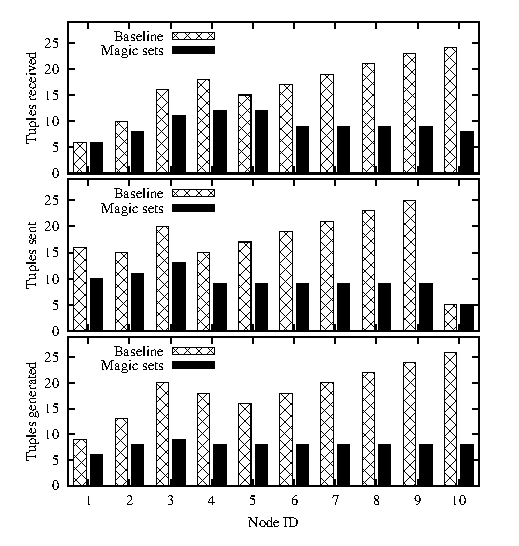
\includegraphics{results/magicNumbers}
\caption{For each node (node ID on $x$ axis), number of tuples received
  (top), sent (middle), and locally generated (bottom) on the $y$ axis.}
\label{fig:magicresults}
\end{figure}



To understand the effects of this rewrite, we describe two experimental
runs of our program, before and after the magic-sets rewrite (both
programs were also subjected to the localization rewrite from
Section~\ref{sec:localization} since they are distributed).  The two
programs are executed in the simple link topology of
Figure~\ref{fig:topo}. Nodes are started up one at a time in order of
identifier, and the preloaded database (EDB) consists of the links pictured. For each experiment we measure the number of
tuples sent and received by each node, as well as any \ol{path}
tuples constructed. The latter measure is meant to convey ``work''
performed by the distributed program even in local computation that does
not appear on the network (e.g., local tuple computations, storage, and
other dependent actions on those tuples).

Figure~\ref{fig:magicresults}(a) shows the number of tuples that each node receives from
the network. The magic-sets rewritten program causes no more tuples to
be received than the original, and for most nodes significantly fewer
when moving to nodes farther away from the clique. That is because many
paths that are generated in the original program with destinations
within the clique other than node $1$ are pruned early on and never
transmitted all the way to the far end.    Similarly,
Figure~\ref{fig:magicresults}(b) shows the number of tuples each node transmits.
Again, the magic-rewritten program does a lot better.  The two programs
have similar tuple transmit/receive overheads for nodes represents the number of tuples a node sends out
over the network. The inclusion of the magic-sets rewrite reduces the number of sends
in all but one case (node $10$). The node with identifier $10$ is the only node with 
no incoming links and 
is therefore never burdened with network traffic other than its
own; as a result, though its received tuple overhead benefits from magic
sets, it transmitted tuple overhead is unaffected, since it already
sends out no extraneous paths other than its sole path towards node $1$.
Finally, tuple storage is impacted beneficially by magic sets everywhere
(Figure~\ref{fig:magicresults}(c)), since
both \ol{path} tuples received from the network, but also those
generated locally for local consumption are pruned away by the rewrite.

% \subsection{Declarative Sensor Networks}
% \label{sec:dsn}

% \petros{Do we really have the space and time for this?}




\subsection{Localization}
\label{sec:localization}

Finally, we briefly describe the localization compiler stage, which turns
a rule with  multiple
location specifiers in its body to many rules, each of which has a
single location specifier in its body; this essentially turns a
distributed join into a set of local joins with partial result
transmissions among the rules involved~\cite{loo-sigmod06}. This rewrite
is part of the P2
system, but implemented in C++ and woven into the monolithic compiler.

In Evita Raced, localization stage traverses distributed rules in
left-to-right order starting with first body predicates (rules with
local-only body predicates are selected out early in the stage). 
The location attribute of the current predicate in this traversal is noted at each iteration.
A {\em breakpoint} is generated if the traversal reaches a predicate with location attribute 
that differs from the previous. The breakpoint triggers a {\em split} rule at the given 
position, which creates a new {\em glue} predicate $IR_p$, and two new rules defined as follows.
\begin{CompactEnumerate}
\item $IR_p$ :- (predicates to the left, excluding the breakpoint).
\item (original rule head predicate) :- $IR_p$, (predicates to the right, including the breakpoint). 
\end{CompactEnumerate}
The location attribute in the $IR_p$ predicate is taken from the predicate at the breakpoint position.
The other attributes in the $IR_p$ predicate are taken from the predicates to the left of (and not 
including) the breakpoint, which represents the schema of the intermediate result prior to the
breakpoint position predicate. The algorithm then removes the original rule, and moves recursively on
the second rule, which is considered the original rule in the above discussion. 
The recursion terminates at the rightmost predicate position. 

The localization stage is not an optimization per se, but rather a  program rewrite necessary to make distributed rules executable. 
% Any program that contains distributed rules must go through this compilation stage. 
The Overlog program for localization consists of only 28 rules. The original P2
code that performed this task in P2 consisted of approximately 400 lines of
% carefully crafted 
C++.  








\section{Related Work}
The pioneering work on extensible query optimizer architectures was done in the EXODUS~\cite{exodus} and Starburst~\cite{lohman,phh92} systems, which provided custom rule languages for specifying plan transformations.  The EXODUS optimizer generator used a forward-chaining rule language to iteratively transform existing query plans into new ones. Follow-on work (Volcano~\cite{volcano} and Cascades~\cite{cascades}) exposed more interfaces to make the search in this space of transformations more efficient.  Starburst had two rule-based optimization stages.  The SQL Query Rewrite stage provided a production rule execution engine, for ``rules'' that were written imperatively in C; it included a precedence ordering facility over those rules.  The cost-based optimizer in Starburst was more declarative, taking a grammar-based approach to specifying legal plans and subplans.

While all of this work was rule-based and extensible, most of it only exposed individual plan transformations to extensibility; the actual search algorithms or transformation orderings of EXODUS, Volcano, Cascades, and the Starburst cost-based optimizer were fixed in procedural code.  By contrast, Evita Raced does not embed a search algorithm, instead leaving that open to specification as needed.  The dynamic programming search we implemented is a natural fit to a Datalog-based rule language, and it is an interesting future work challenge to consider whether the Cascades-style ``top-down'' optimization is easy to achieve in Overlog; the fact that magic-sets rewriting blurs the difference between top-down and bottom-up logic evaluation may be germane here~\cite{topdownbottomup}.

Another interesting extensible query optimizer is Opt++~\cite{kabradewitt}, which exploits the object-oriented features of C++ to make an optimizer framework that was easy to customize in a number of ways.  A specific goal of Opt++ was to make the search strategy extensible, enabling not only top-down vs. bottom-up state-space enumeration, but also randomized search algorithms.  Evita Raced embraces these additional dimensions of extensibility introduced by Opt++, but provides them in a higher-level declarative programming framework.

The cyclic dataflow used for stage scheduling in Evita Races resembles the continuous query engine of TelegraphCQ, with our StageScheduler and Demux elements working together to behave somewhat like the TelegraphCQ {\em eddy} operator~\cite{tcq-cidr}.  This connection occurred to us long after we developed our design, but in retrospect the analogy is quite natural: Evita Raced stages are akin to TelegraphCQ's ``installed'' continuous queries, and P2's Overlog queries are akin to data streaming into TelegraphCQ.

Our description of Overlog was based on our understanding of the current state of the P2 codebase.  Loo et al.~\cite{loo-sigmod06} describe a language for P2 they call Network Datalog (NDLog), that is roughly a simple sub-language of the current state of Overlog.  NDLog is a subset of Datalog with aggregation, and hence does not provide delete rules or updates.  Unlike Overlog, NDLog offers well-defined global program semantics across the network, but it does so by not offering delete or update rules, which are used in many Overlog programs.


\section{Experiences}
\label{sec:gripes}

When we started this work, the vision of declaratively specified
query optimization was appealing thanks to its elegance and its
promise of usability and maintainability.  Although we remain convinced on this front, our optimism has been tempered by the pragmatics of developing software within a
continuously changing system prototype.  Here we reflect on some
of the (hard) lessons we learned while conducting this research.


P2's notion of
consecutive Datalog-style fixpoints, especially in networked
environments, still has many rough edges, both on the design and on the
engineering front.  Because deep down P2's runtime is an event-driven execution
engine, its basic unit of atomicity is akin to a single iteration through a recursive query evaluation strategy like semi-naive evaluation, generating a set of derived actions (tuples to be inserted, deleted, transmitted
remotely, or evaluated locally for further deduction) from a single incoming event, and committing changes to the database atomically upon completion of such a step~\cite{LuThesis}. P2's
Datalog-style fixpoints are implemented as sequences of such
single-event iterations, in a manner that appears to have been an afterthought. As a result, the system's
design shares both 
event-driven and logic-style flavors, with some remaining unresolved
conflicts, and no explicit language constructs to bridge between the two.

One example is the notion of \ol{delete} rules, the semantics of which are unclear.  How is one to handle delete rules triggered by the
\emph{deletion} of a base tuple?  The system certainly does not support
-- semantically or operationally -- the ``undeleting'' of tuples that were
originally deleted due to a base fact that is no longer in the
database.  Similarly, the semantics for multiple updates to
the same tuple within the same fixpoint are undefined and a local tie
breaking rule is chosen to decide on a consistent ordering among
same-fixpoint updates to the same relation. Compiler
stages that do static analysis might catch such dangerous rules and alert the user.

Second, as in most prototypes, the programmer interface is not
polished. Debugging is difficult, especially since the logic language
makes it tough to understand which value corresponds to which formal
attribute in a long tuple of a dozen or more attributes.  Though
concise, declaratively specified optimizations pack a punch in terms of
density of concepts, which only becomes deadlier due to the (otherwise
desirable) arbitrary order of rule execution.  Certainly a better
thought-out system to debug declarative programs -- optimizations, no
less -- would have made the job easier.  To be fair, however, our
experience with building monolithic optimizers in production database
management systems in the past was not a great deal rosier.  It is hard to debug code when the output's correctness (e.g., minimality of cost) is too expensive to verify.

Third, the evolution of the Overlog language has a long way to go. The
language still offers no modularity, making it tough to isolate
and reuse logically distinct components. It does has a rudimentary concrete
type system, but has poor support for structured types like matrices and
lists.  Overlog still ``cuts corners'' on the proper set-orientation
of Datalog; since program stratification is only preliminary in
the system prototype, dealing with streaming aggregates in the face of
EDB updates required us to resort to imperative tricks like timers and
polling to determine that aggregates were ready to be finalized.

Beyond particular characteristics of P2, one hard lesson we learned was
that extensibility and ease of use at the top often comes at the expense of
complexity below the extensibility layer.  The tabularization of
compiler state to enable declarative optimizations also
meant that even imperative compiler stages such as our
bootstrap stages implemented in C++ had to use tables, foregoing their familiar
interaction with C++ data structures.  Building glue libraries that ease
this interaction may relieve this pain.

Nevertheless, despite these complaints, we were able to get all of our desired optimizations expressed in Overlog in a highly compact way, as promised by the various earlier papers on P2.  By contrast, the initial version of P2 had no query optimizations of interest beyond localization.  As Overlog and P2 mature, the use of a metacompilation approach should get even easier.  And based on our initial experience extending Overlog with security properties in a manner similar to~\cite{abadi-netdb07}, we believe that our Evita Raced infrastructure could accelerate the ability of the P2 group to pursue modifications to Overlog itself.

\section{Conclusion and Future Work}
\label{sec:conclude}

The Evita Raced meta-compilation framework allows Overlog program transformations
to be written in Overlog and executed in the P2 query processing engine. The use of metacompilation allowed us to achieve significant code reuse from the core of P2, so that the mechanisms supporting query optimization are a small addition to the core query processing already in the system.  A particularly elegant aspect of this is the scheduling of independent optimization stages by expressing scheduling constraints as data, and having that data processed by a special dataflow element for scheduling.  Our hypothesis that a Datalog-style language was a good fit for typical query optimizations was largely borne out, despite some immaturity in the Overlog language and P2 infrastructure. We were able to express two of the most important optimizer frameworks -- System R and Magic Sets -- in only a few dozen rules each.

Going forward, we hope to exploit the use of a declarative language for benefits beyond code compactness.  The tabularization of the optimizer state is particularly suggestive.  It can be used to enable optimizer debugging via interactive queries or standing alerts (watchpoints) on the optimizer tables.  We are also considering the possibility of implementing adaptive query processing schemes by manipulating the optimizer state, especially given the similarity between our StageScheduler and the eddy operator~\cite{tcq-cidr}.  Evita Raced is fully operational, and on a more pragmatic front we plan to write many additional rewrites in Overlog, including proper program stratification, integrity constraint implementations, and multi-query optimizations.

\bibliographystyle{abbrv}
\bibliography{paper}

\end{document}





% LocalWords:  Overlog Datalog DSN metacompiler declarativity Ullman's fixpoint
% LocalWords:  metacompilation runtime tuples Overlog's tuple liveness Demux
% LocalWords:  programEvent StageLattice StageScheduler demultiplexer tuple's
% LocalWords:  dataflows StageSchedule cardinalities subgoals subplans subplan
% LocalWords:  vertices breakpoint Starburst TelegraphCQ TelegraphCQ's codebase
% LocalWords:  fixpoints undeleting declaratively tabularization
